%!TEX root=main.tex

\section{Experiências}

Foram realizados 2 tipos de experiências distintas. As primeiras experiências foram desenhadas para testar a qualidade das heurísticas implementadas. Isto é, para determinar se os jogadores computador que usam estas heurísticas conseguem atingir bons desempenhos a jogar Pentago. Nomeadamente, tendo duas heurísticas diferentes a jogar Pentago, interessa-nos saber qual ganha. O segundo grupo de experiências pretende determinar qual a eficiência dos algoritmos implementados. Em particular, queremos comparar estes algoritmos entre si.

\subsection{Qualidade das Heurísticas}

Para averiguar a qualidade das heurísticas implementadas foram realizados testes automatizados de computador contra computador e implementada uma heurística de controlo, cujo valor de utilidade que devolve é aleatório. 

As estatísticas apresentadas nesta secção referem-se ao jogador destacado a negrito. Por exemplo, o número de vitórias refere-se a vitórias desse jogador. As vitórias, derrotas, empates e número médio de turnos são representados respetivamente pelas cores azul, vermelha, verde e preta. As três primeiras são apresentadas em permilagem. Todos valores originais foram arredondados para baixo pelo que o somatório das componentes pode n\~ao igualar 1000\perthousand. 

O jogador artificial que jogar com as brancas inicia a partida (ao contrário do Pentago original). 

As informações apresentadas abaixo do nome das heurísticas referem-se aos pesos/opç\~oes usadas. Nas heurísticas 1 e 1.2 são sempre usados (e ocultados nas tabelas) os pesos \verb|default| usados para os diferentes tipos de linhas. Isto porque consideramos que a sua inclusão nos testes não se justifica, dada a reduzida relevância para projeto. Muitas das combinações usadas foram descobertas ao testar, de forma automatizada, as heurísticas com valores pseudo-aleatórios (dentro de determinados intervalos).

Para cada cada heurística os dados apresentados referem-se a:
\begin{itemize}  
	\item 1 - \verb|bias|
	\item 1.2 Relaxada? (Y=sim, N=não); Usa Hack Diagonal? (Y=sim, N=não); possibilidades ; possibilidades para oponente; possibilidades fortes; possibilidades fortes para oponente
	\item A - monica ; meio ; direito ; tripla
	\item A hacked - Pesos da 1.2 ; Pesos da A
	\item A star - Pesos da A ;  Analisa Rotaç\~oes? (Y=sim,N=não)
\end{itemize} 

A primeira ocorrência de uma heurística numa tabela apresenta sempre os pesos \verb|default| da mesma.

Além de testes automáticos foram realizadas também alguns jogos de humano contra as heurísticas implementadas. Para uma profundidade de 4 a heurística A e variantes normalmente conseguem realizar um jogo interessante contra um humano. Ao aumentar a profundidade o jogador humano tem que esperar algum tempo pela resposta, no entanto torna-se muito mais difícil vencer estas heurísticas. 

\subsubsection{Testes de Heurísticas versus Controlo}

Cada teste consiste em 400 partidas com tabuleiro inicial vazio e 400 com tabuleiros aleatórios. Dos 400 tabuleiros aleatórios uma metade são com um número de peças ímpares (jogador com pretas a iniciar a primeira jogada) e a outra metade com um número de peças par (jogador com brancas a iniciar a primeira jogada). 

Repare-se que o valores de referencia para os testes em que a heurística testada joga com as peças pretas devem ser os da heurística de controlo que joga com as peças pretas. Ou seja, para comparar o número de vitórias das heurísticas nestes testes com as de controlo é necessário olhar para as derrotas apresentadas na primeira linha de teste (de controlo contra controlo).

\begin{table}[H]
\centering
\resizebox{\columnwidth}{!} {
\setlength\tabcolsep{ 1.5pt}
\begin{tabular}{|c|c|c|c|c|c|c|c|c|c|c|c|c|c|}
\hline
 &  & \multicolumn{4}{c|}{Tabuleio Inicial Vazio} & \multicolumn{4}{c|}{Tabuleiro Inicial Aleatorio} & \multicolumn{4}{c|}{Total} \\ \cline{3-14}
\multirow{-2}{*}{Joga com Brancas} & \multirow{-2}{*}{Joga com Pretas} & {\color[HTML]{00009B} Vit\perthousand} & {\color[HTML]{9A0000} Der\perthousand} & {\color[HTML]{009901} Emp\perthousand} & Tur & {\color[HTML]{00009B} Vit\perthousand} & {\color[HTML]{9A0000} Der\perthousand} & {\color[HTML]{009901} Emp\perthousand} & Tur & {\color[HTML]{00009B} Vit\perthousand} & {\color[HTML]{9A0000} Der\perthousand} & {\color[HTML]{009901} Emp\perthousand} & Tur \\ \hline

\cellcolor{blue!15}\textbf{control} & control& {\color[HTML]{00009B} } & {\color[HTML]{9A0000} } & {\color[HTML]{009901} } &  & {\color[HTML]{00009B} } & {\color[HTML]{9A0000} } & {\color[HTML]{009901} } &  & {\color[HTML]{00009B} } & {\color[HTML]{9A0000} } & {\color[HTML]{009901} } &  \\ 
\cellcolor{ blue!15} &  & \multirow{-2}{*}{{\color[HTML]{00009B} 627}} & \multirow{-2}{*}{{\color[HTML]{9A0000} 330}} & \multirow{-2}{*}{{\color[HTML]{009901} 42}} & \multirow{-2}{*}{25} & \multirow{-2}{*}{{\color[HTML]{00009B} 660}} & \multirow{-2}{*}{{\color[HTML]{9A0000} 297}} & \multirow{-2}{*}{{\color[HTML]{009901} 42}} & \multirow{-2}{*}{12} & \multirow{-2}{*}{{\color[HTML]{00009B} 643}} & \multirow{-2}{*}{{\color[HTML]{9A0000} 313}} & \multirow{-2}{*}{{\color[HTML]{009901} 42}} & \multirow{-2}{*}{18} \\ \hline

\end{tabular}} \caption{Heurística de Controlo versus Controlo usando Alfa-Beta com profundidade 4 (2 jogadas)} \label{ controlonly } \end{table}
%dv4 tests:200

\begin{table}[H]
\centering
\resizebox{\columnwidth}{!} {
\setlength\tabcolsep{ 1.5pt}
\begin{tabular}{|c|c|c|c|c|c|c|c|c|c|c|c|c|c|}
\hline
 &  & \multicolumn{4}{c|}{Tabuleio Inicial Vazio} & \multicolumn{4}{c|}{Tabuleiro Inicial Aleatorio} & \multicolumn{4}{c|}{Total} \\ \cline{3-14}
\multirow{-2}{*}{Joga com Brancas} & \multirow{-2}{*}{Joga com Pretas} & {\color[HTML]{00009B} Vit\perthousand} & {\color[HTML]{9A0000} Der\perthousand} & {\color[HTML]{009901} Emp\perthousand} & Tur & {\color[HTML]{00009B} Vit\perthousand} & {\color[HTML]{9A0000} Der\perthousand} & {\color[HTML]{009901} Emp\perthousand} & Tur & {\color[HTML]{00009B} Vit\perthousand} & {\color[HTML]{9A0000} Der\perthousand} & {\color[HTML]{009901} Emp\perthousand} & Tur \\ \hline


\cellcolor{blue!15}\textbf{one} & control& {\color[HTML]{00009B} } & {\color[HTML]{9A0000} } & {\color[HTML]{009901} } &  & {\color[HTML]{00009B} } & {\color[HTML]{9A0000} } & {\color[HTML]{009901} } &  & {\color[HTML]{00009B} } & {\color[HTML]{9A0000} } & {\color[HTML]{009901} } &  \\ 
\cellcolor{ blue!15}0,5 &  & \multirow{-2}{*}{{\color[HTML]{00009B} 775}} & \multirow{-2}{*}{{\color[HTML]{9A0000} 170}} & \multirow{-2}{*}{{\color[HTML]{009901} 55}} & \multirow{-2}{*}{23} & \multirow{-2}{*}{{\color[HTML]{00009B} 742}} & \multirow{-2}{*}{{\color[HTML]{9A0000} 175}} & \multirow{-2}{*}{{\color[HTML]{009901} 82}} & \multirow{-2}{*}{12} & \multirow{-2}{*}{{\color[HTML]{00009B} 758}} & \multirow{-2}{*}{{\color[HTML]{9A0000} 172}} & \multirow{-2}{*}{{\color[HTML]{009901} 68}} & \multirow{-2}{*}{17} \\ \hline

control & \cellcolor{blue!15}\textbf{one}& {\color[HTML]{00009B} } & {\color[HTML]{9A0000} } & {\color[HTML]{009901} } &  & {\color[HTML]{00009B} } & {\color[HTML]{9A0000} } & {\color[HTML]{009901} } &  & {\color[HTML]{00009B} } & {\color[HTML]{9A0000} } & {\color[HTML]{009901} } &  \\ 
 & \cellcolor{ blue!15}0,5 & \multirow{-2}{*}{{\color[HTML]{00009B} 482}} & \multirow{-2}{*}{{\color[HTML]{9A0000} 432}} & \multirow{-2}{*}{{\color[HTML]{009901} 85}} & \multirow{-2}{*}{24} & \multirow{-2}{*}{{\color[HTML]{00009B} 377}} & \multirow{-2}{*}{{\color[HTML]{9A0000} 555}} & \multirow{-2}{*}{{\color[HTML]{009901} 67}} & \multirow{-2}{*}{12} & \multirow{-2}{*}{{\color[HTML]{00009B} 430}} & \multirow{-2}{*}{{\color[HTML]{9A0000} 493}} & \multirow{-2}{*}{{\color[HTML]{009901} 76}} & \multirow{-2}{*}{18} \\ \hline

\cellcolor{blue!15}\textbf{one} & control& {\color[HTML]{00009B} } & {\color[HTML]{9A0000} } & {\color[HTML]{009901} } &  & {\color[HTML]{00009B} } & {\color[HTML]{9A0000} } & {\color[HTML]{009901} } &  & {\color[HTML]{00009B} } & {\color[HTML]{9A0000} } & {\color[HTML]{009901} } &  \\ 
\cellcolor{ blue!15}0 &  & \multirow{-2}{*}{{\color[HTML]{00009B} 762}} & \multirow{-2}{*}{{\color[HTML]{9A0000} 105}} & \multirow{-2}{*}{{\color[HTML]{009901} 132}} & \multirow{-2}{*}{24} & \multirow{-2}{*}{{\color[HTML]{00009B} 712}} & \multirow{-2}{*}{{\color[HTML]{9A0000} 185}} & \multirow{-2}{*}{{\color[HTML]{009901} 102}} & \multirow{-2}{*}{12} & \multirow{-2}{*}{{\color[HTML]{00009B} 737}} & \multirow{-2}{*}{{\color[HTML]{9A0000} 145}} & \multirow{-2}{*}{{\color[HTML]{009901} 117}} & \multirow{-2}{*}{18} \\ \hline

control & \cellcolor{blue!15}\textbf{one}& {\color[HTML]{00009B} } & {\color[HTML]{9A0000} } & {\color[HTML]{009901} } &  & {\color[HTML]{00009B} } & {\color[HTML]{9A0000} } & {\color[HTML]{009901} } &  & {\color[HTML]{00009B} } & {\color[HTML]{9A0000} } & {\color[HTML]{009901} } &  \\ 
 & \cellcolor{ blue!15}0 & \multirow{-2}{*}{{\color[HTML]{00009B} 475}} & \multirow{-2}{*}{{\color[HTML]{9A0000} 355}} & \multirow{-2}{*}{{\color[HTML]{009901} 170}} & \multirow{-2}{*}{24} & \multirow{-2}{*}{{\color[HTML]{00009B} 352}} & \multirow{-2}{*}{{\color[HTML]{9A0000} 530}} & \multirow{-2}{*}{{\color[HTML]{009901} 117}} & \multirow{-2}{*}{13} & \multirow{-2}{*}{{\color[HTML]{00009B} 413}} & \multirow{-2}{*}{{\color[HTML]{9A0000} 442}} & \multirow{-2}{*}{{\color[HTML]{009901} 143}} & \multirow{-2}{*}{18} \\ \hline

\cellcolor{blue!15}\textbf{one} & control& {\color[HTML]{00009B} } & {\color[HTML]{9A0000} } & {\color[HTML]{009901} } &  & {\color[HTML]{00009B} } & {\color[HTML]{9A0000} } & {\color[HTML]{009901} } &  & {\color[HTML]{00009B} } & {\color[HTML]{9A0000} } & {\color[HTML]{009901} } &  \\ 
\cellcolor{ blue!15}1 &  & \multirow{-2}{*}{{\color[HTML]{00009B} 695}} & \multirow{-2}{*}{{\color[HTML]{9A0000} 255}} & \multirow{-2}{*}{{\color[HTML]{009901} 50}} & \multirow{-2}{*}{23} & \multirow{-2}{*}{{\color[HTML]{00009B} 770}} & \multirow{-2}{*}{{\color[HTML]{9A0000} 217}} & \multirow{-2}{*}{{\color[HTML]{009901} 12}} & \multirow{-2}{*}{11} & \multirow{-2}{*}{{\color[HTML]{00009B} 732}} & \multirow{-2}{*}{{\color[HTML]{9A0000} 236}} & \multirow{-2}{*}{{\color[HTML]{009901} 31}} & \multirow{-2}{*}{17} \\ \hline

control & \cellcolor{blue!15}\textbf{one}& {\color[HTML]{00009B} } & {\color[HTML]{9A0000} } & {\color[HTML]{009901} } &  & {\color[HTML]{00009B} } & {\color[HTML]{9A0000} } & {\color[HTML]{009901} } &  & {\color[HTML]{00009B} } & {\color[HTML]{9A0000} } & {\color[HTML]{009901} } &  \\ 
 & \cellcolor{ blue!15}1 & \multirow{-2}{*}{{\color[HTML]{00009B} 427}} & \multirow{-2}{*}{{\color[HTML]{9A0000} 542}} & \multirow{-2}{*}{{\color[HTML]{009901} 30}} & \multirow{-2}{*}{23} & \multirow{-2}{*}{{\color[HTML]{00009B} 365}} & \multirow{-2}{*}{{\color[HTML]{9A0000} 620}} & \multirow{-2}{*}{{\color[HTML]{009901} 15}} & \multirow{-2}{*}{11} & \multirow{-2}{*}{{\color[HTML]{00009B} 396}} & \multirow{-2}{*}{{\color[HTML]{9A0000} 581}} & \multirow{-2}{*}{{\color[HTML]{009901} 22}} & \multirow{-2}{*}{17} \\ \hline


\cellcolor{blue!15}\textbf{oneDotTwo} & control& {\color[HTML]{00009B} } & {\color[HTML]{9A0000} } & {\color[HTML]{009901} } &  & {\color[HTML]{00009B} } & {\color[HTML]{9A0000} } & {\color[HTML]{009901} } &  & {\color[HTML]{00009B} } & {\color[HTML]{9A0000} } & {\color[HTML]{009901} } &  \\ 
\cellcolor{ blue!15}R:Y ; DH:N ; 1 ; 1 ; 1 ; 1 &  & \multirow{-2}{*}{{\color[HTML]{00009B} 787}} & \multirow{-2}{*}{{\color[HTML]{9A0000} 157}} & \multirow{-2}{*}{{\color[HTML]{009901} 55}} & \multirow{-2}{*}{23} & \multirow{-2}{*}{{\color[HTML]{00009B} 767}} & \multirow{-2}{*}{{\color[HTML]{9A0000} 175}} & \multirow{-2}{*}{{\color[HTML]{009901} 57}} & \multirow{-2}{*}{12} & \multirow{-2}{*}{{\color[HTML]{00009B} 777}} & \multirow{-2}{*}{{\color[HTML]{9A0000} 166}} & \multirow{-2}{*}{{\color[HTML]{009901} 56}} & \multirow{-2}{*}{17} \\ \hline

\cellcolor{blue!15}\textbf{oneDotTwo} & control& {\color[HTML]{00009B} } & {\color[HTML]{9A0000} } & {\color[HTML]{009901} } &  & {\color[HTML]{00009B} } & {\color[HTML]{9A0000} } & {\color[HTML]{009901} } &  & {\color[HTML]{00009B} } & {\color[HTML]{9A0000} } & {\color[HTML]{009901} } &  \\ 
\cellcolor{ blue!15}R:Y ; DH:N ; 4 ; 3 ; 2 ; 8 &  & \multirow{-2}{*}{{\color[HTML]{00009B} 790}} & \multirow{-2}{*}{{\color[HTML]{9A0000} 112}} & \multirow{-2}{*}{{\color[HTML]{009901} 97}} & \multirow{-2}{*}{24} & \multirow{-2}{*}{{\color[HTML]{00009B} 760}} & \multirow{-2}{*}{{\color[HTML]{9A0000} 152}} & \multirow{-2}{*}{{\color[HTML]{009901} 87}} & \multirow{-2}{*}{13} & \multirow{-2}{*}{{\color[HTML]{00009B} 775}} & \multirow{-2}{*}{{\color[HTML]{9A0000} 132}} & \multirow{-2}{*}{{\color[HTML]{009901} 92}} & \multirow{-2}{*}{18} \\ \hline

\cellcolor{blue!15}\textbf{oneDotTwo} & control& {\color[HTML]{00009B} } & {\color[HTML]{9A0000} } & {\color[HTML]{009901} } &  & {\color[HTML]{00009B} } & {\color[HTML]{9A0000} } & {\color[HTML]{009901} } &  & {\color[HTML]{00009B} } & {\color[HTML]{9A0000} } & {\color[HTML]{009901} } &  \\ 
\cellcolor{ blue!15}R:Y ; DH:N ; 3 ; 4 ; 8 ; 3 &  & \multirow{-2}{*}{{\color[HTML]{00009B} 685}} & \multirow{-2}{*}{{\color[HTML]{9A0000} 250}} & \multirow{-2}{*}{{\color[HTML]{009901} 65}} & \multirow{-2}{*}{26} & \multirow{-2}{*}{{\color[HTML]{00009B} 750}} & \multirow{-2}{*}{{\color[HTML]{9A0000} 190}} & \multirow{-2}{*}{{\color[HTML]{009901} 60}} & \multirow{-2}{*}{12} & \multirow{-2}{*}{{\color[HTML]{00009B} 717}} & \multirow{-2}{*}{{\color[HTML]{9A0000} 220}} & \multirow{-2}{*}{{\color[HTML]{009901} 62}} & \multirow{-2}{*}{19} \\ \hline

\cellcolor{blue!15}\textbf{oneDotTwo} & control& {\color[HTML]{00009B} } & {\color[HTML]{9A0000} } & {\color[HTML]{009901} } &  & {\color[HTML]{00009B} } & {\color[HTML]{9A0000} } & {\color[HTML]{009901} } &  & {\color[HTML]{00009B} } & {\color[HTML]{9A0000} } & {\color[HTML]{009901} } &  \\ 
\cellcolor{ blue!15}R:Y ; DH:N ; 1 ; 5 ; 3 ; 10,1 &  & \multirow{-2}{*}{{\color[HTML]{00009B} 805}} & \multirow{-2}{*}{{\color[HTML]{9A0000} 97}} & \multirow{-2}{*}{{\color[HTML]{009901} 97}} & \multirow{-2}{*}{24} & \multirow{-2}{*}{{\color[HTML]{00009B} 732}} & \multirow{-2}{*}{{\color[HTML]{9A0000} 185}} & \multirow{-2}{*}{{\color[HTML]{009901} 82}} & \multirow{-2}{*}{12} & \multirow{-2}{*}{{\color[HTML]{00009B} 768}} & \multirow{-2}{*}{{\color[HTML]{9A0000} 141}} & \multirow{-2}{*}{{\color[HTML]{009901} 90}} & \multirow{-2}{*}{18} \\ \hline

\cellcolor{blue!15}\textbf{oneDotTwo} & control& {\color[HTML]{00009B} } & {\color[HTML]{9A0000} } & {\color[HTML]{009901} } &  & {\color[HTML]{00009B} } & {\color[HTML]{9A0000} } & {\color[HTML]{009901} } &  & {\color[HTML]{00009B} } & {\color[HTML]{9A0000} } & {\color[HTML]{009901} } &  \\ 
\cellcolor{ blue!15}R:Y ; DH:N ; 5 ; 1 ; 8,1 ; 3 &  & \multirow{-2}{*}{{\color[HTML]{00009B} 730}} & \multirow{-2}{*}{{\color[HTML]{9A0000} 205}} & \multirow{-2}{*}{{\color[HTML]{009901} 65}} & \multirow{-2}{*}{25} & \multirow{-2}{*}{{\color[HTML]{00009B} 755}} & \multirow{-2}{*}{{\color[HTML]{9A0000} 207}} & \multirow{-2}{*}{{\color[HTML]{009901} 37}} & \multirow{-2}{*}{12} & \multirow{-2}{*}{{\color[HTML]{00009B} 742}} & \multirow{-2}{*}{{\color[HTML]{9A0000} 206}} & \multirow{-2}{*}{{\color[HTML]{009901} 51}} & \multirow{-2}{*}{18} \\ \hline

\cellcolor{blue!15}\textbf{oneDotTwo} & control& {\color[HTML]{00009B} } & {\color[HTML]{9A0000} } & {\color[HTML]{009901} } &  & {\color[HTML]{00009B} } & {\color[HTML]{9A0000} } & {\color[HTML]{009901} } &  & {\color[HTML]{00009B} } & {\color[HTML]{9A0000} } & {\color[HTML]{009901} } &  \\ 
\cellcolor{ blue!15}R:Y ; DH:N ; 10 ; 10 ; 6 ; 4 &  & \multirow{-2}{*}{{\color[HTML]{00009B} 795}} & \multirow{-2}{*}{{\color[HTML]{9A0000} 170}} & \multirow{-2}{*}{{\color[HTML]{009901} 35}} & \multirow{-2}{*}{23} & \multirow{-2}{*}{{\color[HTML]{00009B} 727}} & \multirow{-2}{*}{{\color[HTML]{9A0000} 192}} & \multirow{-2}{*}{{\color[HTML]{009901} 80}} & \multirow{-2}{*}{12} & \multirow{-2}{*}{{\color[HTML]{00009B} 761}} & \multirow{-2}{*}{{\color[HTML]{9A0000} 181}} & \multirow{-2}{*}{{\color[HTML]{009901} 57}} & \multirow{-2}{*}{17} \\ \hline

control & \cellcolor{blue!15}\textbf{oneDotTwo}& {\color[HTML]{00009B} } & {\color[HTML]{9A0000} } & {\color[HTML]{009901} } &  & {\color[HTML]{00009B} } & {\color[HTML]{9A0000} } & {\color[HTML]{009901} } &  & {\color[HTML]{00009B} } & {\color[HTML]{9A0000} } & {\color[HTML]{009901} } &  \\ 
 & \cellcolor{ blue!15}R:Y ; DH:N ; 1 ; 1 ; 1 ; 1 & \multirow{-2}{*}{{\color[HTML]{00009B} 650}} & \multirow{-2}{*}{{\color[HTML]{9A0000} 300}} & \multirow{-2}{*}{{\color[HTML]{009901} 50}} & \multirow{-2}{*}{22} & \multirow{-2}{*}{{\color[HTML]{00009B} 412}} & \multirow{-2}{*}{{\color[HTML]{9A0000} 520}} & \multirow{-2}{*}{{\color[HTML]{009901} 67}} & \multirow{-2}{*}{12} & \multirow{-2}{*}{{\color[HTML]{00009B} 531}} & \multirow{-2}{*}{{\color[HTML]{9A0000} 410}} & \multirow{-2}{*}{{\color[HTML]{009901} 58}} & \multirow{-2}{*}{17} \\ \hline

control & \cellcolor{blue!15}\textbf{oneDotTwo}& {\color[HTML]{00009B} } & {\color[HTML]{9A0000} } & {\color[HTML]{009901} } &  & {\color[HTML]{00009B} } & {\color[HTML]{9A0000} } & {\color[HTML]{009901} } &  & {\color[HTML]{00009B} } & {\color[HTML]{9A0000} } & {\color[HTML]{009901} } &  \\ 
 & \cellcolor{ blue!15}R:Y ; DH:N ; 4 ; 3 ; 2 ; 8 & \multirow{-2}{*}{{\color[HTML]{00009B} 475}} & \multirow{-2}{*}{{\color[HTML]{9A0000} 405}} & \multirow{-2}{*}{{\color[HTML]{009901} 120}} & \multirow{-2}{*}{26} & \multirow{-2}{*}{{\color[HTML]{00009B} 322}} & \multirow{-2}{*}{{\color[HTML]{9A0000} 585}} & \multirow{-2}{*}{{\color[HTML]{009901} 92}} & \multirow{-2}{*}{13} & \multirow{-2}{*}{{\color[HTML]{00009B} 398}} & \multirow{-2}{*}{{\color[HTML]{9A0000} 495}} & \multirow{-2}{*}{{\color[HTML]{009901} 106}} & \multirow{-2}{*}{19} \\ \hline

control & \cellcolor{blue!15}\textbf{oneDotTwo}& {\color[HTML]{00009B} } & {\color[HTML]{9A0000} } & {\color[HTML]{009901} } &  & {\color[HTML]{00009B} } & {\color[HTML]{9A0000} } & {\color[HTML]{009901} } &  & {\color[HTML]{00009B} } & {\color[HTML]{9A0000} } & {\color[HTML]{009901} } &  \\ 
 & \cellcolor{ blue!15}R:Y ; DH:N ; 3 ; 4 ; 8 ; 3 & \multirow{-2}{*}{{\color[HTML]{00009B} 835}} & \multirow{-2}{*}{{\color[HTML]{9A0000} 155}} & \multirow{-2}{*}{{\color[HTML]{009901} 10}} & \multirow{-2}{*}{18} & \multirow{-2}{*}{{\color[HTML]{00009B} 480}} & \multirow{-2}{*}{{\color[HTML]{9A0000} 477}} & \multirow{-2}{*}{{\color[HTML]{009901} 42}} & \multirow{-2}{*}{11} & \multirow{-2}{*}{{\color[HTML]{00009B} 657}} & \multirow{-2}{*}{{\color[HTML]{9A0000} 316}} & \multirow{-2}{*}{{\color[HTML]{009901} 26}} & \multirow{-2}{*}{14} \\ \hline

control & \cellcolor{blue!15}\textbf{oneDotTwo}& {\color[HTML]{00009B} } & {\color[HTML]{9A0000} } & {\color[HTML]{009901} } &  & {\color[HTML]{00009B} } & {\color[HTML]{9A0000} } & {\color[HTML]{009901} } &  & {\color[HTML]{00009B} } & {\color[HTML]{9A0000} } & {\color[HTML]{009901} } &  \\ 
 & \cellcolor{ blue!15}R:Y ; DH:N ; 1 ; 5 ; 3 ; 10,1 & \multirow{-2}{*}{{\color[HTML]{00009B} 510}} & \multirow{-2}{*}{{\color[HTML]{9A0000} 382}} & \multirow{-2}{*}{{\color[HTML]{009901} 107}} & \multirow{-2}{*}{26} & \multirow{-2}{*}{{\color[HTML]{00009B} 365}} & \multirow{-2}{*}{{\color[HTML]{9A0000} 552}} & \multirow{-2}{*}{{\color[HTML]{009901} 82}} & \multirow{-2}{*}{13} & \multirow{-2}{*}{{\color[HTML]{00009B} 437}} & \multirow{-2}{*}{{\color[HTML]{9A0000} 467}} & \multirow{-2}{*}{{\color[HTML]{009901} 95}} & \multirow{-2}{*}{19} \\ \hline

control & \cellcolor{blue!15}\textbf{oneDotTwo}& {\color[HTML]{00009B} } & {\color[HTML]{9A0000} } & {\color[HTML]{009901} } &  & {\color[HTML]{00009B} } & {\color[HTML]{9A0000} } & {\color[HTML]{009901} } &  & {\color[HTML]{00009B} } & {\color[HTML]{9A0000} } & {\color[HTML]{009901} } &  \\ 
 & \cellcolor{ blue!15}R:Y ; DH:N ; 5 ; 1 ; 8,1 ; 3 & \multirow{-2}{*}{{\color[HTML]{00009B} 482}} & \multirow{-2}{*}{{\color[HTML]{9A0000} 495}} & \multirow{-2}{*}{{\color[HTML]{009901} 22}} & \multirow{-2}{*}{22} & \multirow{-2}{*}{{\color[HTML]{00009B} 370}} & \multirow{-2}{*}{{\color[HTML]{9A0000} 590}} & \multirow{-2}{*}{{\color[HTML]{009901} 40}} & \multirow{-2}{*}{12} & \multirow{-2}{*}{{\color[HTML]{00009B} 426}} & \multirow{-2}{*}{{\color[HTML]{9A0000} 542}} & \multirow{-2}{*}{{\color[HTML]{009901} 31}} & \multirow{-2}{*}{17} \\ \hline

control & \cellcolor{blue!15}\textbf{oneDotTwo}& {\color[HTML]{00009B} } & {\color[HTML]{9A0000} } & {\color[HTML]{009901} } &  & {\color[HTML]{00009B} } & {\color[HTML]{9A0000} } & {\color[HTML]{009901} } &  & {\color[HTML]{00009B} } & {\color[HTML]{9A0000} } & {\color[HTML]{009901} } &  \\ 
 & \cellcolor{ blue!15}R:Y ; DH:N ; 10 ; 10 ; 6 ; 4 & \multirow{-2}{*}{{\color[HTML]{00009B} 522}} & \multirow{-2}{*}{{\color[HTML]{9A0000} 442}} & \multirow{-2}{*}{{\color[HTML]{009901} 35}} & \multirow{-2}{*}{23} & \multirow{-2}{*}{{\color[HTML]{00009B} 395}} & \multirow{-2}{*}{{\color[HTML]{9A0000} 535}} & \multirow{-2}{*}{{\color[HTML]{009901} 70}} & \multirow{-2}{*}{12} & \multirow{-2}{*}{{\color[HTML]{00009B} 458}} & \multirow{-2}{*}{{\color[HTML]{9A0000} 488}} & \multirow{-2}{*}{{\color[HTML]{009901} 52}} & \multirow{-2}{*}{17} \\ \hline
\end{tabular}} \caption{Heurística '1' e variantes versus Controlo usando Alfa-Beta com profundidade 4 (2 jogadas)} \label{onecontrol} \end{table}

%===========================================
%===========================================
%===========================================

%dv4 tests:200

\begin{table}[H]
\centering
\resizebox{\columnwidth}{!} {
\setlength\tabcolsep{ 1.5pt}
\begin{tabular}{|c|c|c|c|c|c|c|c|c|c|c|c|c|c|}
\hline
 &  & \multicolumn{4}{c|}{Tabuleio Inicial Vazio} & \multicolumn{4}{c|}{Tabuleiro Inicial Aleatorio} & \multicolumn{4}{c|}{Total} \\ \cline{3-14}
\multirow{-2}{*}{Joga com Brancas} & \multirow{-2}{*}{Joga com Pretas} & {\color[HTML]{00009B} Vit\perthousand} & {\color[HTML]{9A0000} Der\perthousand} & {\color[HTML]{009901} Emp\perthousand} & Tur & {\color[HTML]{00009B} Vit\perthousand} & {\color[HTML]{9A0000} Der\perthousand} & {\color[HTML]{009901} Emp\perthousand} & Tur & {\color[HTML]{00009B} Vit\perthousand} & {\color[HTML]{9A0000} Der\perthousand} & {\color[HTML]{009901} Emp\perthousand} & Tur \\ \hline


\cellcolor{blue!15}\textbf{A} & control& {\color[HTML]{00009B} } & {\color[HTML]{9A0000} } & {\color[HTML]{009901} } &  & {\color[HTML]{00009B} } & {\color[HTML]{9A0000} } & {\color[HTML]{009901} } &  & {\color[HTML]{00009B} } & {\color[HTML]{9A0000} } & {\color[HTML]{009901} } &  \\ 
\cellcolor{ blue!15}1,13 ; 1,15 ; 1,17 ; 1,19 &  & \multirow{-2}{*}{{\color[HTML]{00009B} 977}} & \multirow{-2}{*}{{\color[HTML]{9A0000} 20}} & \multirow{-2}{*}{{\color[HTML]{009901} 2}} & \multirow{-2}{*}{17} & \multirow{-2}{*}{{\color[HTML]{00009B} 905}} & \multirow{-2}{*}{{\color[HTML]{9A0000} 67}} & \multirow{-2}{*}{{\color[HTML]{009901} 27}} & \multirow{-2}{*}{8} & \multirow{-2}{*}{{\color[HTML]{00009B} 941}} & \multirow{-2}{*}{{\color[HTML]{9A0000} 43}} & \multirow{-2}{*}{{\color[HTML]{009901} 15}} & \multirow{-2}{*}{12} \\ \hline

\cellcolor{blue!15}\textbf{A} & control& {\color[HTML]{00009B} } & {\color[HTML]{9A0000} } & {\color[HTML]{009901} } &  & {\color[HTML]{00009B} } & {\color[HTML]{9A0000} } & {\color[HTML]{009901} } &  & {\color[HTML]{00009B} } & {\color[HTML]{9A0000} } & {\color[HTML]{009901} } &  \\ 
\cellcolor{ blue!15}1,23308 ; 1,26326 ; 1,11807 ; 0,99693 &  & \multirow{-2}{*}{{\color[HTML]{00009B} 997}} & \multirow{-2}{*}{{\color[HTML]{9A0000} 2}} & \multirow{-2}{*}{{\color[HTML]{009901} 0}} & \multirow{-2}{*}{13} & \multirow{-2}{*}{{\color[HTML]{00009B} 912}} & \multirow{-2}{*}{{\color[HTML]{9A0000} 67}} & \multirow{-2}{*}{{\color[HTML]{009901} 20}} & \multirow{-2}{*}{6} & \multirow{-2}{*}{{\color[HTML]{00009B} 955}} & \multirow{-2}{*}{{\color[HTML]{9A0000} 35}} & \multirow{-2}{*}{{\color[HTML]{009901} 10}} & \multirow{-2}{*}{9} \\ \hline

\cellcolor{blue!15}\textbf{A} & control& {\color[HTML]{00009B} } & {\color[HTML]{9A0000} } & {\color[HTML]{009901} } &  & {\color[HTML]{00009B} } & {\color[HTML]{9A0000} } & {\color[HTML]{009901} } &  & {\color[HTML]{00009B} } & {\color[HTML]{9A0000} } & {\color[HTML]{009901} } &  \\ 
\cellcolor{ blue!15}0,946981 ; 1,120938 ; 1,126149 ; 1,23813 &  & \multirow{-2}{*}{{\color[HTML]{00009B} 940}} & \multirow{-2}{*}{{\color[HTML]{9A0000} 40}} & \multirow{-2}{*}{{\color[HTML]{009901} 20}} & \multirow{-2}{*}{20} & \multirow{-2}{*}{{\color[HTML]{00009B} 902}} & \multirow{-2}{*}{{\color[HTML]{9A0000} 80}} & \multirow{-2}{*}{{\color[HTML]{009901} 17}} & \multirow{-2}{*}{9} & \multirow{-2}{*}{{\color[HTML]{00009B} 921}} & \multirow{-2}{*}{{\color[HTML]{9A0000} 60}} & \multirow{-2}{*}{{\color[HTML]{009901} 18}} & \multirow{-2}{*}{14} \\ \hline

\cellcolor{blue!15}\textbf{A} & control& {\color[HTML]{00009B} } & {\color[HTML]{9A0000} } & {\color[HTML]{009901} } &  & {\color[HTML]{00009B} } & {\color[HTML]{9A0000} } & {\color[HTML]{009901} } &  & {\color[HTML]{00009B} } & {\color[HTML]{9A0000} } & {\color[HTML]{009901} } &  \\ 
\cellcolor{ blue!15}0,917492 ; 1,138074 ; 1,259564 ; 1,168299 &  & \multirow{-2}{*}{{\color[HTML]{00009B} 950}} & \multirow{-2}{*}{{\color[HTML]{9A0000} 35}} & \multirow{-2}{*}{{\color[HTML]{009901} 15}} & \multirow{-2}{*}{21} & \multirow{-2}{*}{{\color[HTML]{00009B} 895}} & \multirow{-2}{*}{{\color[HTML]{9A0000} 80}} & \multirow{-2}{*}{{\color[HTML]{009901} 25}} & \multirow{-2}{*}{10} & \multirow{-2}{*}{{\color[HTML]{00009B} 922}} & \multirow{-2}{*}{{\color[HTML]{9A0000} 57}} & \multirow{-2}{*}{{\color[HTML]{009901} 20}} & \multirow{-2}{*}{15} \\ \hline

control & \cellcolor{blue!15}\textbf{A}& {\color[HTML]{00009B} } & {\color[HTML]{9A0000} } & {\color[HTML]{009901} } &  & {\color[HTML]{00009B} } & {\color[HTML]{9A0000} } & {\color[HTML]{009901} } &  & {\color[HTML]{00009B} } & {\color[HTML]{9A0000} } & {\color[HTML]{009901} } &  \\ 
 & \cellcolor{ blue!15}1,13 ; 1,15 ; 1,17 ; 1,19 & \multirow{-2}{*}{{\color[HTML]{00009B} 912}} & \multirow{-2}{*}{{\color[HTML]{9A0000} 72}} & \multirow{-2}{*}{{\color[HTML]{009901} 15}} & \multirow{-2}{*}{20} & \multirow{-2}{*}{{\color[HTML]{00009B} 697}} & \multirow{-2}{*}{{\color[HTML]{9A0000} 265}} & \multirow{-2}{*}{{\color[HTML]{009901} 37}} & \multirow{-2}{*}{9} & \multirow{-2}{*}{{\color[HTML]{00009B} 805}} & \multirow{-2}{*}{{\color[HTML]{9A0000} 168}} & \multirow{-2}{*}{{\color[HTML]{009901} 26}} & \multirow{-2}{*}{14} \\ \hline

control & \cellcolor{blue!15}\textbf{A}& {\color[HTML]{00009B} } & {\color[HTML]{9A0000} } & {\color[HTML]{009901} } &  & {\color[HTML]{00009B} } & {\color[HTML]{9A0000} } & {\color[HTML]{009901} } &  & {\color[HTML]{00009B} } & {\color[HTML]{9A0000} } & {\color[HTML]{009901} } &  \\ 
 & \cellcolor{ blue!15}1,23308 ; 1,26326 ; 1,11807 ; 0,99693 & \multirow{-2}{*}{{\color[HTML]{00009B} 992}} & \multirow{-2}{*}{{\color[HTML]{9A0000} 5}} & \multirow{-2}{*}{{\color[HTML]{009901} 2}} & \multirow{-2}{*}{14} & \multirow{-2}{*}{{\color[HTML]{00009B} 717}} & \multirow{-2}{*}{{\color[HTML]{9A0000} 252}} & \multirow{-2}{*}{{\color[HTML]{009901} 30}} & \multirow{-2}{*}{7} & \multirow{-2}{*}{{\color[HTML]{00009B} 855}} & \multirow{-2}{*}{{\color[HTML]{9A0000} 128}} & \multirow{-2}{*}{{\color[HTML]{009901} 16}} & \multirow{-2}{*}{10} \\ \hline

control & \cellcolor{blue!15}\textbf{A}& {\color[HTML]{00009B} } & {\color[HTML]{9A0000} } & {\color[HTML]{009901} } &  & {\color[HTML]{00009B} } & {\color[HTML]{9A0000} } & {\color[HTML]{009901} } &  & {\color[HTML]{00009B} } & {\color[HTML]{9A0000} } & {\color[HTML]{009901} } &  \\ 
 & \cellcolor{ blue!15}0,946981 ; 1,120938 ; 1,126149 ; 1,23813 & \multirow{-2}{*}{{\color[HTML]{00009B} 847}} & \multirow{-2}{*}{{\color[HTML]{9A0000} 122}} & \multirow{-2}{*}{{\color[HTML]{009901} 30}} & \multirow{-2}{*}{22} & \multirow{-2}{*}{{\color[HTML]{00009B} 687}} & \multirow{-2}{*}{{\color[HTML]{9A0000} 280}} & \multirow{-2}{*}{{\color[HTML]{009901} 32}} & \multirow{-2}{*}{10} & \multirow{-2}{*}{{\color[HTML]{00009B} 767}} & \multirow{-2}{*}{{\color[HTML]{9A0000} 201}} & \multirow{-2}{*}{{\color[HTML]{009901} 31}} & \multirow{-2}{*}{16} \\ \hline

control & \cellcolor{blue!15}\textbf{A}& {\color[HTML]{00009B} } & {\color[HTML]{9A0000} } & {\color[HTML]{009901} } &  & {\color[HTML]{00009B} } & {\color[HTML]{9A0000} } & {\color[HTML]{009901} } &  & {\color[HTML]{00009B} } & {\color[HTML]{9A0000} } & {\color[HTML]{009901} } &  \\ 
 & \cellcolor{ blue!15}0,917492 ; 1,138074 ; 1,259564 ; 1,168299 & \multirow{-2}{*}{{\color[HTML]{00009B} 775}} & \multirow{-2}{*}{{\color[HTML]{9A0000} 170}} & \multirow{-2}{*}{{\color[HTML]{009901} 55}} & \multirow{-2}{*}{23} & \multirow{-2}{*}{{\color[HTML]{00009B} 612}} & \multirow{-2}{*}{{\color[HTML]{9A0000} 335}} & \multirow{-2}{*}{{\color[HTML]{009901} 52}} & \multirow{-2}{*}{11} & \multirow{-2}{*}{{\color[HTML]{00009B} 693}} & \multirow{-2}{*}{{\color[HTML]{9A0000} 252}} & \multirow{-2}{*}{{\color[HTML]{009901} 53}} & \multirow{-2}{*}{17} \\ \hline


\cellcolor{blue!15}\textbf{Astar} & control& {\color[HTML]{00009B} } & {\color[HTML]{9A0000} } & {\color[HTML]{009901} } &  & {\color[HTML]{00009B} } & {\color[HTML]{9A0000} } & {\color[HTML]{009901} } &  & {\color[HTML]{00009B} } & {\color[HTML]{9A0000} } & {\color[HTML]{009901} } &  \\ 
\cellcolor{ blue!15}1,13 ; 1,15 ; 1,17 ; 1,19 ; Y &  & \multirow{-2}{*}{{\color[HTML]{00009B} 985}} & \multirow{-2}{*}{{\color[HTML]{9A0000} 7}} & \multirow{-2}{*}{{\color[HTML]{009901} 7}} & \multirow{-2}{*}{11} & \multirow{-2}{*}{{\color[HTML]{00009B} 897}} & \multirow{-2}{*}{{\color[HTML]{9A0000} 67}} & \multirow{-2}{*}{{\color[HTML]{009901} 35}} & \multirow{-2}{*}{6} & \multirow{-2}{*}{{\color[HTML]{00009B} 941}} & \multirow{-2}{*}{{\color[HTML]{9A0000} 37}} & \multirow{-2}{*}{{\color[HTML]{009901} 21}} & \multirow{-2}{*}{8} \\ \hline

\cellcolor{blue!15}\textbf{Astar} & control& {\color[HTML]{00009B} } & {\color[HTML]{9A0000} } & {\color[HTML]{009901} } &  & {\color[HTML]{00009B} } & {\color[HTML]{9A0000} } & {\color[HTML]{009901} } &  & {\color[HTML]{00009B} } & {\color[HTML]{9A0000} } & {\color[HTML]{009901} } &  \\ 
\cellcolor{ blue!15}1,23308 ; 1,26326 ; 1,11807 ; 0,99693 ; Y &  & \multirow{-2}{*}{{\color[HTML]{00009B} 1000}} & \multirow{-2}{*}{{\color[HTML]{9A0000} 0}} & \multirow{-2}{*}{{\color[HTML]{009901} 0}} & \multirow{-2}{*}{9} & \multirow{-2}{*}{{\color[HTML]{00009B} 907}} & \multirow{-2}{*}{{\color[HTML]{9A0000} 65}} & \multirow{-2}{*}{{\color[HTML]{009901} 27}} & \multirow{-2}{*}{6} & \multirow{-2}{*}{{\color[HTML]{00009B} 953}} & \multirow{-2}{*}{{\color[HTML]{9A0000} 32}} & \multirow{-2}{*}{{\color[HTML]{009901} 13}} & \multirow{-2}{*}{7} \\ \hline

\cellcolor{blue!15}\textbf{Astar} & control& {\color[HTML]{00009B} } & {\color[HTML]{9A0000} } & {\color[HTML]{009901} } &  & {\color[HTML]{00009B} } & {\color[HTML]{9A0000} } & {\color[HTML]{009901} } &  & {\color[HTML]{00009B} } & {\color[HTML]{9A0000} } & {\color[HTML]{009901} } &  \\ 
\cellcolor{ blue!15}0,946981 ; 1,120938 ; 1,126149 ; 1,23813 ; Y &  & \multirow{-2}{*}{{\color[HTML]{00009B} 980}} & \multirow{-2}{*}{{\color[HTML]{9A0000} 10}} & \multirow{-2}{*}{{\color[HTML]{009901} 10}} & \multirow{-2}{*}{15} & \multirow{-2}{*}{{\color[HTML]{00009B} 897}} & \multirow{-2}{*}{{\color[HTML]{9A0000} 70}} & \multirow{-2}{*}{{\color[HTML]{009901} 32}} & \multirow{-2}{*}{7} & \multirow{-2}{*}{{\color[HTML]{00009B} 938}} & \multirow{-2}{*}{{\color[HTML]{9A0000} 40}} & \multirow{-2}{*}{{\color[HTML]{009901} 21}} & \multirow{-2}{*}{11} \\ \hline

\cellcolor{blue!15}\textbf{Astar} & control& {\color[HTML]{00009B} } & {\color[HTML]{9A0000} } & {\color[HTML]{009901} } &  & {\color[HTML]{00009B} } & {\color[HTML]{9A0000} } & {\color[HTML]{009901} } &  & {\color[HTML]{00009B} } & {\color[HTML]{9A0000} } & {\color[HTML]{009901} } &  \\ 
\cellcolor{ blue!15}0,917492 ; 1,138074 ; 1,259564 ; 1,168299 ; Y &  & \multirow{-2}{*}{{\color[HTML]{00009B} 985}} & \multirow{-2}{*}{{\color[HTML]{9A0000} 7}} & \multirow{-2}{*}{{\color[HTML]{009901} 7}} & \multirow{-2}{*}{14} & \multirow{-2}{*}{{\color[HTML]{00009B} 902}} & \multirow{-2}{*}{{\color[HTML]{9A0000} 67}} & \multirow{-2}{*}{{\color[HTML]{009901} 30}} & \multirow{-2}{*}{7} & \multirow{-2}{*}{{\color[HTML]{00009B} 943}} & \multirow{-2}{*}{{\color[HTML]{9A0000} 37}} & \multirow{-2}{*}{{\color[HTML]{009901} 18}} & \multirow{-2}{*}{10} \\ \hline

control & \cellcolor{blue!15}\textbf{Astar}& {\color[HTML]{00009B} } & {\color[HTML]{9A0000} } & {\color[HTML]{009901} } &  & {\color[HTML]{00009B} } & {\color[HTML]{9A0000} } & {\color[HTML]{009901} } &  & {\color[HTML]{00009B} } & {\color[HTML]{9A0000} } & {\color[HTML]{009901} } &  \\ 
 & \cellcolor{ blue!15}1,13 ; 1,15 ; 1,17 ; 1,19 ; Y & \multirow{-2}{*}{{\color[HTML]{00009B} 982}} & \multirow{-2}{*}{{\color[HTML]{9A0000} 12}} & \multirow{-2}{*}{{\color[HTML]{009901} 5}} & \multirow{-2}{*}{12} & \multirow{-2}{*}{{\color[HTML]{00009B} 712}} & \multirow{-2}{*}{{\color[HTML]{9A0000} 245}} & \multirow{-2}{*}{{\color[HTML]{009901} 42}} & \multirow{-2}{*}{7} & \multirow{-2}{*}{{\color[HTML]{00009B} 847}} & \multirow{-2}{*}{{\color[HTML]{9A0000} 128}} & \multirow{-2}{*}{{\color[HTML]{009901} 23}} & \multirow{-2}{*}{9} \\ \hline

control & \cellcolor{blue!15}\textbf{Astar}& {\color[HTML]{00009B} } & {\color[HTML]{9A0000} } & {\color[HTML]{009901} } &  & {\color[HTML]{00009B} } & {\color[HTML]{9A0000} } & {\color[HTML]{009901} } &  & {\color[HTML]{00009B} } & {\color[HTML]{9A0000} } & {\color[HTML]{009901} } &  \\ 
 & \cellcolor{ blue!15}1,23308 ; 1,26326 ; 1,11807 ; 0,99693 ; Y & \multirow{-2}{*}{{\color[HTML]{00009B} 1000}} & \multirow{-2}{*}{{\color[HTML]{9A0000} 0}} & \multirow{-2}{*}{{\color[HTML]{009901} 0}} & \multirow{-2}{*}{11} & \multirow{-2}{*}{{\color[HTML]{00009B} 742}} & \multirow{-2}{*}{{\color[HTML]{9A0000} 220}} & \multirow{-2}{*}{{\color[HTML]{009901} 37}} & \multirow{-2}{*}{7} & \multirow{-2}{*}{{\color[HTML]{00009B} 871}} & \multirow{-2}{*}{{\color[HTML]{9A0000} 110}} & \multirow{-2}{*}{{\color[HTML]{009901} 18}} & \multirow{-2}{*}{9} \\ \hline

control & \cellcolor{blue!15}\textbf{Astar}& {\color[HTML]{00009B} } & {\color[HTML]{9A0000} } & {\color[HTML]{009901} } &  & {\color[HTML]{00009B} } & {\color[HTML]{9A0000} } & {\color[HTML]{009901} } &  & {\color[HTML]{00009B} } & {\color[HTML]{9A0000} } & {\color[HTML]{009901} } &  \\ 
 & \cellcolor{ blue!15}0,946981 ; 1,120938 ; 1,126149 ; 1,23813 ; Y & \multirow{-2}{*}{{\color[HTML]{00009B} 920}} & \multirow{-2}{*}{{\color[HTML]{9A0000} 52}} & \multirow{-2}{*}{{\color[HTML]{009901} 27}} & \multirow{-2}{*}{18} & \multirow{-2}{*}{{\color[HTML]{00009B} 705}} & \multirow{-2}{*}{{\color[HTML]{9A0000} 232}} & \multirow{-2}{*}{{\color[HTML]{009901} 62}} & \multirow{-2}{*}{8} & \multirow{-2}{*}{{\color[HTML]{00009B} 812}} & \multirow{-2}{*}{{\color[HTML]{9A0000} 142}} & \multirow{-2}{*}{{\color[HTML]{009901} 45}} & \multirow{-2}{*}{13} \\ \hline

control & \cellcolor{blue!15}\textbf{Astar}& {\color[HTML]{00009B} } & {\color[HTML]{9A0000} } & {\color[HTML]{009901} } &  & {\color[HTML]{00009B} } & {\color[HTML]{9A0000} } & {\color[HTML]{009901} } &  & {\color[HTML]{00009B} } & {\color[HTML]{9A0000} } & {\color[HTML]{009901} } &  \\ 
 & \cellcolor{ blue!15}0,917492 ; 1,138074 ; 1,259564 ; 1,168299 ; Y & \multirow{-2}{*}{{\color[HTML]{00009B} 922}} & \multirow{-2}{*}{{\color[HTML]{9A0000} 45}} & \multirow{-2}{*}{{\color[HTML]{009901} 32}} & \multirow{-2}{*}{16} & \multirow{-2}{*}{{\color[HTML]{00009B} 660}} & \multirow{-2}{*}{{\color[HTML]{9A0000} 265}} & \multirow{-2}{*}{{\color[HTML]{009901} 75}} & \multirow{-2}{*}{9} & \multirow{-2}{*}{{\color[HTML]{00009B} 791}} & \multirow{-2}{*}{{\color[HTML]{9A0000} 155}} & \multirow{-2}{*}{{\color[HTML]{009901} 53}} & \multirow{-2}{*}{12} \\ \hline


\cellcolor{blue!15}\textbf{AplusDiagHack} & control& {\color[HTML]{00009B} } & {\color[HTML]{9A0000} } & {\color[HTML]{009901} } &  & {\color[HTML]{00009B} } & {\color[HTML]{9A0000} } & {\color[HTML]{009901} } &  & {\color[HTML]{00009B} } & {\color[HTML]{9A0000} } & {\color[HTML]{009901} } &  \\ 
\cellcolor{ blue!15}0 ; 0 ; 1 ; 0 ; 1,13 ; 1,15 ; 1,17 ; 1,19 &  & \multirow{-2}{*}{{\color[HTML]{00009B} 975}} & \multirow{-2}{*}{{\color[HTML]{9A0000} 15}} & \multirow{-2}{*}{{\color[HTML]{009901} 10}} & \multirow{-2}{*}{16} & \multirow{-2}{*}{{\color[HTML]{00009B} 887}} & \multirow{-2}{*}{{\color[HTML]{9A0000} 70}} & \multirow{-2}{*}{{\color[HTML]{009901} 42}} & \multirow{-2}{*}{8} & \multirow{-2}{*}{{\color[HTML]{00009B} 931}} & \multirow{-2}{*}{{\color[HTML]{9A0000} 42}} & \multirow{-2}{*}{{\color[HTML]{009901} 26}} & \multirow{-2}{*}{12} \\ \hline

\cellcolor{blue!15}\textbf{AplusDiagHack} & control& {\color[HTML]{00009B} } & {\color[HTML]{9A0000} } & {\color[HTML]{009901} } &  & {\color[HTML]{00009B} } & {\color[HTML]{9A0000} } & {\color[HTML]{009901} } &  & {\color[HTML]{00009B} } & {\color[HTML]{9A0000} } & {\color[HTML]{009901} } &  \\ 
\cellcolor{ blue!15}0 ; 0 ; 1 ; 0 ; 1,23308 ; 1,26326 ; 1,11807 ; 0,99693 &  & \multirow{-2}{*}{{\color[HTML]{00009B} 965}} & \multirow{-2}{*}{{\color[HTML]{9A0000} 22}} & \multirow{-2}{*}{{\color[HTML]{009901} 12}} & \multirow{-2}{*}{14} & \multirow{-2}{*}{{\color[HTML]{00009B} 882}} & \multirow{-2}{*}{{\color[HTML]{9A0000} 87}} & \multirow{-2}{*}{{\color[HTML]{009901} 30}} & \multirow{-2}{*}{7} & \multirow{-2}{*}{{\color[HTML]{00009B} 923}} & \multirow{-2}{*}{{\color[HTML]{9A0000} 55}} & \multirow{-2}{*}{{\color[HTML]{009901} 21}} & \multirow{-2}{*}{10} \\ \hline

\cellcolor{blue!15}\textbf{AplusDiagHack} & control& {\color[HTML]{00009B} } & {\color[HTML]{9A0000} } & {\color[HTML]{009901} } &  & {\color[HTML]{00009B} } & {\color[HTML]{9A0000} } & {\color[HTML]{009901} } &  & {\color[HTML]{00009B} } & {\color[HTML]{9A0000} } & {\color[HTML]{009901} } &  \\ 
\cellcolor{ blue!15}0 ; 0 ; 1 ; 0 ; 0,946981 ; 1,120938 ; 1,126149 ; 1,23813 &  & \multirow{-2}{*}{{\color[HTML]{00009B} 950}} & \multirow{-2}{*}{{\color[HTML]{9A0000} 35}} & \multirow{-2}{*}{{\color[HTML]{009901} 15}} & \multirow{-2}{*}{18} & \multirow{-2}{*}{{\color[HTML]{00009B} 895}} & \multirow{-2}{*}{{\color[HTML]{9A0000} 80}} & \multirow{-2}{*}{{\color[HTML]{009901} 25}} & \multirow{-2}{*}{9} & \multirow{-2}{*}{{\color[HTML]{00009B} 922}} & \multirow{-2}{*}{{\color[HTML]{9A0000} 57}} & \multirow{-2}{*}{{\color[HTML]{009901} 20}} & \multirow{-2}{*}{13} \\ \hline

\cellcolor{blue!15}\textbf{AplusDiagHack} & control& {\color[HTML]{00009B} } & {\color[HTML]{9A0000} } & {\color[HTML]{009901} } &  & {\color[HTML]{00009B} } & {\color[HTML]{9A0000} } & {\color[HTML]{009901} } &  & {\color[HTML]{00009B} } & {\color[HTML]{9A0000} } & {\color[HTML]{009901} } &  \\ 
\cellcolor{ blue!15}0 ; 0 ; 1 ; 0 ; 0,917492 ; 1,138074 ; 1,259564 ; 1,168299 &  & \multirow{-2}{*}{{\color[HTML]{00009B} 935}} & \multirow{-2}{*}{{\color[HTML]{9A0000} 37}} & \multirow{-2}{*}{{\color[HTML]{009901} 27}} & \multirow{-2}{*}{19} & \multirow{-2}{*}{{\color[HTML]{00009B} 877}} & \multirow{-2}{*}{{\color[HTML]{9A0000} 95}} & \multirow{-2}{*}{{\color[HTML]{009901} 27}} & \multirow{-2}{*}{9} & \multirow{-2}{*}{{\color[HTML]{00009B} 906}} & \multirow{-2}{*}{{\color[HTML]{9A0000} 66}} & \multirow{-2}{*}{{\color[HTML]{009901} 27}} & \multirow{-2}{*}{14} \\ \hline

control & \cellcolor{blue!15}\textbf{AplusDiagHack}& {\color[HTML]{00009B} } & {\color[HTML]{9A0000} } & {\color[HTML]{009901} } &  & {\color[HTML]{00009B} } & {\color[HTML]{9A0000} } & {\color[HTML]{009901} } &  & {\color[HTML]{00009B} } & {\color[HTML]{9A0000} } & {\color[HTML]{009901} } &  \\ 
 & \cellcolor{ blue!15}0 ; 0 ; 1 ; 2 ; 1,13 ; 1,15 ; 1,17 ; 1,19 & \multirow{-2}{*}{{\color[HTML]{00009B} 912}} & \multirow{-2}{*}{{\color[HTML]{9A0000} 60}} & \multirow{-2}{*}{{\color[HTML]{009901} 27}} & \multirow{-2}{*}{18} & \multirow{-2}{*}{{\color[HTML]{00009B} 745}} & \multirow{-2}{*}{{\color[HTML]{9A0000} 227}} & \multirow{-2}{*}{{\color[HTML]{009901} 27}} & \multirow{-2}{*}{9} & \multirow{-2}{*}{{\color[HTML]{00009B} 828}} & \multirow{-2}{*}{{\color[HTML]{9A0000} 143}} & \multirow{-2}{*}{{\color[HTML]{009901} 27}} & \multirow{-2}{*}{13} \\ \hline

control & \cellcolor{blue!15}\textbf{AplusDiagHack}& {\color[HTML]{00009B} } & {\color[HTML]{9A0000} } & {\color[HTML]{009901} } &  & {\color[HTML]{00009B} } & {\color[HTML]{9A0000} } & {\color[HTML]{009901} } &  & {\color[HTML]{00009B} } & {\color[HTML]{9A0000} } & {\color[HTML]{009901} } &  \\ 
 & \cellcolor{ blue!15}0 ; 0 ; 1 ; 2 ; 1,23308 ; 1,26326 ; 1,11807 ; 0,99693 & \multirow{-2}{*}{{\color[HTML]{00009B} 975}} & \multirow{-2}{*}{{\color[HTML]{9A0000} 20}} & \multirow{-2}{*}{{\color[HTML]{009901} 5}} & \multirow{-2}{*}{13} & \multirow{-2}{*}{{\color[HTML]{00009B} 720}} & \multirow{-2}{*}{{\color[HTML]{9A0000} 260}} & \multirow{-2}{*}{{\color[HTML]{009901} 20}} & \multirow{-2}{*}{7} & \multirow{-2}{*}{{\color[HTML]{00009B} 847}} & \multirow{-2}{*}{{\color[HTML]{9A0000} 140}} & \multirow{-2}{*}{{\color[HTML]{009901} 12}} & \multirow{-2}{*}{10} \\ \hline

control & \cellcolor{blue!15}\textbf{AplusDiagHack}& {\color[HTML]{00009B} } & {\color[HTML]{9A0000} } & {\color[HTML]{009901} } &  & {\color[HTML]{00009B} } & {\color[HTML]{9A0000} } & {\color[HTML]{009901} } &  & {\color[HTML]{00009B} } & {\color[HTML]{9A0000} } & {\color[HTML]{009901} } &  \\ 
 & \cellcolor{ blue!15}0 ; 0 ; 1 ; 2 ; 0,946981 ; 1,120938 ; 1,126149 ; 1,23813 & \multirow{-2}{*}{{\color[HTML]{00009B} 880}} & \multirow{-2}{*}{{\color[HTML]{9A0000} 80}} & \multirow{-2}{*}{{\color[HTML]{009901} 40}} & \multirow{-2}{*}{20} & \multirow{-2}{*}{{\color[HTML]{00009B} 645}} & \multirow{-2}{*}{{\color[HTML]{9A0000} 310}} & \multirow{-2}{*}{{\color[HTML]{009901} 45}} & \multirow{-2}{*}{9} & \multirow{-2}{*}{{\color[HTML]{00009B} 762}} & \multirow{-2}{*}{{\color[HTML]{9A0000} 195}} & \multirow{-2}{*}{{\color[HTML]{009901} 42}} & \multirow{-2}{*}{14} \\ \hline

control & \cellcolor{blue!15}\textbf{AplusDiagHack}& {\color[HTML]{00009B} } & {\color[HTML]{9A0000} } & {\color[HTML]{009901} } &  & {\color[HTML]{00009B} } & {\color[HTML]{9A0000} } & {\color[HTML]{009901} } &  & {\color[HTML]{00009B} } & {\color[HTML]{9A0000} } & {\color[HTML]{009901} } &  \\ 
 & \cellcolor{ blue!15}0 ; 0 ; 1 ; 2 ; 0,917492 ; 1,138074 ; 1,259564 ; 1,168299 & \multirow{-2}{*}{{\color[HTML]{00009B} 780}} & \multirow{-2}{*}{{\color[HTML]{9A0000} 172}} & \multirow{-2}{*}{{\color[HTML]{009901} 47}} & \multirow{-2}{*}{23} & \multirow{-2}{*}{{\color[HTML]{00009B} 672}} & \multirow{-2}{*}{{\color[HTML]{9A0000} 292}} & \multirow{-2}{*}{{\color[HTML]{009901} 35}} & \multirow{-2}{*}{10} & \multirow{-2}{*}{{\color[HTML]{00009B} 726}} & \multirow{-2}{*}{{\color[HTML]{9A0000} 232}} & \multirow{-2}{*}{{\color[HTML]{009901} 41}} & \multirow{-2}{*}{16} \\ \hline
\end{tabular}} \caption{Heurística A e variantes versus Controlo usando Alfa-Beta com profundidade 4 (2 jogadas)} \label{Acontrol} \end{table}


\newpage
\subsubsection{Testes de Heurísticas versus Heurísticas}

Cada teste consiste em 200 partidas com tabuleiro inicial vazio e 200 com tabuleiros aleatórios. Dos 200 tabuleiros aleatórios uma metade são com um número de peças ímpares (jogador com pretas a iniciar a primeira jogada) e a outra metade com um número de peças par (jogador com brancas a iniciar a primeira jogada).

%dv4 tests:100

\begin{table}[H]
\centering
\resizebox{\columnwidth}{!} {
\setlength\tabcolsep{ 1.5pt}
\begin{tabular}{|c|c|c|c|c|c|c|c|c|c|c|c|c|c|}
\hline
 &  & \multicolumn{4}{c|}{Tabuleio Inicial Vazio} & \multicolumn{4}{c|}{Tabuleiro Inicial Aleatorio} & \multicolumn{4}{c|}{Total} \\ \cline{3-14}
\multirow{-2}{*}{Joga com Brancas} & \multirow{-2}{*}{Joga com Pretas} & {\color[HTML]{00009B} Vit\perthousand} & {\color[HTML]{9A0000} Der\perthousand} & {\color[HTML]{009901} Emp\perthousand} & Tur & {\color[HTML]{00009B} Vit\perthousand} & {\color[HTML]{9A0000} Der\perthousand} & {\color[HTML]{009901} Emp\perthousand} & Tur & {\color[HTML]{00009B} Vit\perthousand} & {\color[HTML]{9A0000} Der\perthousand} & {\color[HTML]{009901} Emp\perthousand} & Tur \\ \hline

\cellcolor{blue!15}\textbf{A} & A& {\color[HTML]{00009B} } & {\color[HTML]{9A0000} } & {\color[HTML]{009901} } &  & {\color[HTML]{00009B} } & {\color[HTML]{9A0000} } & {\color[HTML]{009901} } &  & {\color[HTML]{00009B} } & {\color[HTML]{9A0000} } & {\color[HTML]{009901} } &  \\ 
\cellcolor{ blue!15}1,13 ; 1,15 ; 1,17 ; 1,19 & 1,13 ; 1,15 ; 1,17 ; 1,19 & \multirow{-2}{*}{{\color[HTML]{00009B} 420}} & \multirow{-2}{*}{{\color[HTML]{9A0000} 535}} & \multirow{-2}{*}{{\color[HTML]{009901} 45}} & \multirow{-2}{*}{21} & \multirow{-2}{*}{{\color[HTML]{00009B} 540}} & \multirow{-2}{*}{{\color[HTML]{9A0000} 385}} & \multirow{-2}{*}{{\color[HTML]{009901} 75}} & \multirow{-2}{*}{9} & \multirow{-2}{*}{{\color[HTML]{00009B} 480}} & \multirow{-2}{*}{{\color[HTML]{9A0000} 460}} & \multirow{-2}{*}{{\color[HTML]{009901} 60}} & \multirow{-2}{*}{15} \\ \hline

\cellcolor{blue!15}\textbf{A} & Astar& {\color[HTML]{00009B} } & {\color[HTML]{9A0000} } & {\color[HTML]{009901} } &  & {\color[HTML]{00009B} } & {\color[HTML]{9A0000} } & {\color[HTML]{009901} } &  & {\color[HTML]{00009B} } & {\color[HTML]{9A0000} } & {\color[HTML]{009901} } &  \\ 
\cellcolor{ blue!15}1,13 ; 1,15 ; 1,17 ; 1,19 & 1,13 ; 1,15 ; 1,17 ; 1,19 ; Y & \multirow{-2}{*}{{\color[HTML]{00009B} 670}} & \multirow{-2}{*}{{\color[HTML]{9A0000} 325}} & \multirow{-2}{*}{{\color[HTML]{009901} 5}} & \multirow{-2}{*}{21} & \multirow{-2}{*}{{\color[HTML]{00009B} 405}} & \multirow{-2}{*}{{\color[HTML]{9A0000} 520}} & \multirow{-2}{*}{{\color[HTML]{009901} 75}} & \multirow{-2}{*}{8} & \multirow{-2}{*}{{\color[HTML]{00009B} 537}} & \multirow{-2}{*}{{\color[HTML]{9A0000} 422}} & \multirow{-2}{*}{{\color[HTML]{009901} 40}} & \multirow{-2}{*}{14} \\ \hline

\cellcolor{blue!15}\textbf{A} & one& {\color[HTML]{00009B} } & {\color[HTML]{9A0000} } & {\color[HTML]{009901} } &  & {\color[HTML]{00009B} } & {\color[HTML]{9A0000} } & {\color[HTML]{009901} } &  & {\color[HTML]{00009B} } & {\color[HTML]{9A0000} } & {\color[HTML]{009901} } &  \\ 
\cellcolor{ blue!15}1,13 ; 1,15 ; 1,17 ; 1,19 & 0,5 & \multirow{-2}{*}{{\color[HTML]{00009B} 900}} & \multirow{-2}{*}{{\color[HTML]{9A0000} 55}} & \multirow{-2}{*}{{\color[HTML]{009901} 45}} & \multirow{-2}{*}{20} & \multirow{-2}{*}{{\color[HTML]{00009B} 745}} & \multirow{-2}{*}{{\color[HTML]{9A0000} 180}} & \multirow{-2}{*}{{\color[HTML]{009901} 75}} & \multirow{-2}{*}{9} & \multirow{-2}{*}{{\color[HTML]{00009B} 822}} & \multirow{-2}{*}{{\color[HTML]{9A0000} 117}} & \multirow{-2}{*}{{\color[HTML]{009901} 60}} & \multirow{-2}{*}{14} \\ \hline

\cellcolor{blue!15}\textbf{A} & oneDotTwo& {\color[HTML]{00009B} } & {\color[HTML]{9A0000} } & {\color[HTML]{009901} } &  & {\color[HTML]{00009B} } & {\color[HTML]{9A0000} } & {\color[HTML]{009901} } &  & {\color[HTML]{00009B} } & {\color[HTML]{9A0000} } & {\color[HTML]{009901} } &  \\ 
\cellcolor{ blue!15}1,13 ; 1,15 ; 1,17 ; 1,19 & R:Y ; DH:N ; 1 ; 1 ; 1 ; 1 & \multirow{-2}{*}{{\color[HTML]{00009B} 815}} & \multirow{-2}{*}{{\color[HTML]{9A0000} 120}} & \multirow{-2}{*}{{\color[HTML]{009901} 65}} & \multirow{-2}{*}{22} & \multirow{-2}{*}{{\color[HTML]{00009B} 765}} & \multirow{-2}{*}{{\color[HTML]{9A0000} 185}} & \multirow{-2}{*}{{\color[HTML]{009901} 50}} & \multirow{-2}{*}{9} & \multirow{-2}{*}{{\color[HTML]{00009B} 790}} & \multirow{-2}{*}{{\color[HTML]{9A0000} 152}} & \multirow{-2}{*}{{\color[HTML]{009901} 57}} & \multirow{-2}{*}{15} \\ \hline

\cellcolor{blue!15}\textbf{A} & AplusDiagHack& {\color[HTML]{00009B} } & {\color[HTML]{9A0000} } & {\color[HTML]{009901} } &  & {\color[HTML]{00009B} } & {\color[HTML]{9A0000} } & {\color[HTML]{009901} } &  & {\color[HTML]{00009B} } & {\color[HTML]{9A0000} } & {\color[HTML]{009901} } &  \\ 
\cellcolor{ blue!15}1,13 ; 1,15 ; 1,17 ; 1,19 & 0 ; 0 ; 1 ; 2 ; 1,13 ; 1,15 ; 1,17 ; 1,19 & \multirow{-2}{*}{{\color[HTML]{00009B} 0}} & \multirow{-2}{*}{{\color[HTML]{9A0000} 990}} & \multirow{-2}{*}{{\color[HTML]{009901} 10}} & \multirow{-2}{*}{16} & \multirow{-2}{*}{{\color[HTML]{00009B} 500}} & \multirow{-2}{*}{{\color[HTML]{9A0000} 415}} & \multirow{-2}{*}{{\color[HTML]{009901} 85}} & \multirow{-2}{*}{9} & \multirow{-2}{*}{{\color[HTML]{00009B} 250}} & \multirow{-2}{*}{{\color[HTML]{9A0000} 702}} & \multirow{-2}{*}{{\color[HTML]{009901} 47}} & \multirow{-2}{*}{12} \\ \hline

\cellcolor{blue!15}\textbf{Astar} & A& {\color[HTML]{00009B} } & {\color[HTML]{9A0000} } & {\color[HTML]{009901} } &  & {\color[HTML]{00009B} } & {\color[HTML]{9A0000} } & {\color[HTML]{009901} } &  & {\color[HTML]{00009B} } & {\color[HTML]{9A0000} } & {\color[HTML]{009901} } &  \\ 
\cellcolor{ blue!15}1,13 ; 1,15 ; 1,17 ; 1,19 ; Y & 1,13 ; 1,15 ; 1,17 ; 1,19 & \multirow{-2}{*}{{\color[HTML]{00009B} 425}} & \multirow{-2}{*}{{\color[HTML]{9A0000} 530}} & \multirow{-2}{*}{{\color[HTML]{009901} 45}} & \multirow{-2}{*}{24} & \multirow{-2}{*}{{\color[HTML]{00009B} 600}} & \multirow{-2}{*}{{\color[HTML]{9A0000} 320}} & \multirow{-2}{*}{{\color[HTML]{009901} 80}} & \multirow{-2}{*}{7} & \multirow{-2}{*}{{\color[HTML]{00009B} 512}} & \multirow{-2}{*}{{\color[HTML]{9A0000} 425}} & \multirow{-2}{*}{{\color[HTML]{009901} 62}} & \multirow{-2}{*}{15} \\ \hline

\cellcolor{blue!15}\textbf{Astar} & Astar& {\color[HTML]{00009B} } & {\color[HTML]{9A0000} } & {\color[HTML]{009901} } &  & {\color[HTML]{00009B} } & {\color[HTML]{9A0000} } & {\color[HTML]{009901} } &  & {\color[HTML]{00009B} } & {\color[HTML]{9A0000} } & {\color[HTML]{009901} } &  \\ 
\cellcolor{ blue!15}1,13 ; 1,15 ; 1,17 ; 1,19 ; Y & 1,13 ; 1,15 ; 1,17 ; 1,19 ; Y & \multirow{-2}{*}{{\color[HTML]{00009B} 915}} & \multirow{-2}{*}{{\color[HTML]{9A0000} 60}} & \multirow{-2}{*}{{\color[HTML]{009901} 25}} & \multirow{-2}{*}{11} & \multirow{-2}{*}{{\color[HTML]{00009B} 530}} & \multirow{-2}{*}{{\color[HTML]{9A0000} 390}} & \multirow{-2}{*}{{\color[HTML]{009901} 80}} & \multirow{-2}{*}{8} & \multirow{-2}{*}{{\color[HTML]{00009B} 722}} & \multirow{-2}{*}{{\color[HTML]{9A0000} 225}} & \multirow{-2}{*}{{\color[HTML]{009901} 52}} & \multirow{-2}{*}{9} \\ \hline

\cellcolor{blue!15}\textbf{Astar} & one& {\color[HTML]{00009B} } & {\color[HTML]{9A0000} } & {\color[HTML]{009901} } &  & {\color[HTML]{00009B} } & {\color[HTML]{9A0000} } & {\color[HTML]{009901} } &  & {\color[HTML]{00009B} } & {\color[HTML]{9A0000} } & {\color[HTML]{009901} } &  \\ 
\cellcolor{ blue!15}1,13 ; 1,15 ; 1,17 ; 1,19 ; Y & 0,5 & \multirow{-2}{*}{{\color[HTML]{00009B} 970}} & \multirow{-2}{*}{{\color[HTML]{9A0000} 0}} & \multirow{-2}{*}{{\color[HTML]{009901} 30}} & \multirow{-2}{*}{16} & \multirow{-2}{*}{{\color[HTML]{00009B} 790}} & \multirow{-2}{*}{{\color[HTML]{9A0000} 165}} & \multirow{-2}{*}{{\color[HTML]{009901} 45}} & \multirow{-2}{*}{7} & \multirow{-2}{*}{{\color[HTML]{00009B} 880}} & \multirow{-2}{*}{{\color[HTML]{9A0000} 82}} & \multirow{-2}{*}{{\color[HTML]{009901} 37}} & \multirow{-2}{*}{11} \\ \hline

\cellcolor{blue!15}\textbf{Astar} & oneDotTwo& {\color[HTML]{00009B} } & {\color[HTML]{9A0000} } & {\color[HTML]{009901} } &  & {\color[HTML]{00009B} } & {\color[HTML]{9A0000} } & {\color[HTML]{009901} } &  & {\color[HTML]{00009B} } & {\color[HTML]{9A0000} } & {\color[HTML]{009901} } &  \\ 
\cellcolor{ blue!15}1,13 ; 1,15 ; 1,17 ; 1,19 ; Y & R:Y ; DH:N ; 1 ; 1 ; 1 ; 1 & \multirow{-2}{*}{{\color[HTML]{00009B} 615}} & \multirow{-2}{*}{{\color[HTML]{9A0000} 370}} & \multirow{-2}{*}{{\color[HTML]{009901} 15}} & \multirow{-2}{*}{14} & \multirow{-2}{*}{{\color[HTML]{00009B} 790}} & \multirow{-2}{*}{{\color[HTML]{9A0000} 165}} & \multirow{-2}{*}{{\color[HTML]{009901} 45}} & \multirow{-2}{*}{7} & \multirow{-2}{*}{{\color[HTML]{00009B} 702}} & \multirow{-2}{*}{{\color[HTML]{9A0000} 267}} & \multirow{-2}{*}{{\color[HTML]{009901} 30}} & \multirow{-2}{*}{10} \\ \hline

\cellcolor{blue!15}\textbf{Astar} & AplusDiagHack& {\color[HTML]{00009B} } & {\color[HTML]{9A0000} } & {\color[HTML]{009901} } &  & {\color[HTML]{00009B} } & {\color[HTML]{9A0000} } & {\color[HTML]{009901} } &  & {\color[HTML]{00009B} } & {\color[HTML]{9A0000} } & {\color[HTML]{009901} } &  \\ 
\cellcolor{ blue!15}1,13 ; 1,15 ; 1,17 ; 1,19 ; Y & 0 ; 0 ; 1 ; 2 ; 1,13 ; 1,15 ; 1,17 ; 1,19 & \multirow{-2}{*}{{\color[HTML]{00009B} 685}} & \multirow{-2}{*}{{\color[HTML]{9A0000} 315}} & \multirow{-2}{*}{{\color[HTML]{009901} 0}} & \multirow{-2}{*}{14} & \multirow{-2}{*}{{\color[HTML]{00009B} 605}} & \multirow{-2}{*}{{\color[HTML]{9A0000} 300}} & \multirow{-2}{*}{{\color[HTML]{009901} 95}} & \multirow{-2}{*}{7} & \multirow{-2}{*}{{\color[HTML]{00009B} 645}} & \multirow{-2}{*}{{\color[HTML]{9A0000} 307}} & \multirow{-2}{*}{{\color[HTML]{009901} 47}} & \multirow{-2}{*}{10} \\ \hline

\cellcolor{blue!15}\textbf{one} & A& {\color[HTML]{00009B} } & {\color[HTML]{9A0000} } & {\color[HTML]{009901} } &  & {\color[HTML]{00009B} } & {\color[HTML]{9A0000} } & {\color[HTML]{009901} } &  & {\color[HTML]{00009B} } & {\color[HTML]{9A0000} } & {\color[HTML]{009901} } &  \\ 
\cellcolor{ blue!15}0,5 & 1,13 ; 1,15 ; 1,17 ; 1,19 & \multirow{-2}{*}{{\color[HTML]{00009B} 250}} & \multirow{-2}{*}{{\color[HTML]{9A0000} 650}} & \multirow{-2}{*}{{\color[HTML]{009901} 100}} & \multirow{-2}{*}{22} & \multirow{-2}{*}{{\color[HTML]{00009B} 290}} & \multirow{-2}{*}{{\color[HTML]{9A0000} 655}} & \multirow{-2}{*}{{\color[HTML]{009901} 55}} & \multirow{-2}{*}{9} & \multirow{-2}{*}{{\color[HTML]{00009B} 270}} & \multirow{-2}{*}{{\color[HTML]{9A0000} 652}} & \multirow{-2}{*}{{\color[HTML]{009901} 77}} & \multirow{-2}{*}{15} \\ \hline

\cellcolor{blue!15}\textbf{one} & Astar& {\color[HTML]{00009B} } & {\color[HTML]{9A0000} } & {\color[HTML]{009901} } &  & {\color[HTML]{00009B} } & {\color[HTML]{9A0000} } & {\color[HTML]{009901} } &  & {\color[HTML]{00009B} } & {\color[HTML]{9A0000} } & {\color[HTML]{009901} } &  \\ 
\cellcolor{ blue!15}0,5 & 1,13 ; 1,15 ; 1,17 ; 1,19 ; Y & \multirow{-2}{*}{{\color[HTML]{00009B} 5}} & \multirow{-2}{*}{{\color[HTML]{9A0000} 995}} & \multirow{-2}{*}{{\color[HTML]{009901} 0}} & \multirow{-2}{*}{12} & \multirow{-2}{*}{{\color[HTML]{00009B} 160}} & \multirow{-2}{*}{{\color[HTML]{9A0000} 790}} & \multirow{-2}{*}{{\color[HTML]{009901} 50}} & \multirow{-2}{*}{7} & \multirow{-2}{*}{{\color[HTML]{00009B} 82}} & \multirow{-2}{*}{{\color[HTML]{9A0000} 892}} & \multirow{-2}{*}{{\color[HTML]{009901} 25}} & \multirow{-2}{*}{9} \\ \hline

\cellcolor{blue!15}\textbf{one} & one& {\color[HTML]{00009B} } & {\color[HTML]{9A0000} } & {\color[HTML]{009901} } &  & {\color[HTML]{00009B} } & {\color[HTML]{9A0000} } & {\color[HTML]{009901} } &  & {\color[HTML]{00009B} } & {\color[HTML]{9A0000} } & {\color[HTML]{009901} } &  \\ 
\cellcolor{ blue!15}0,5 & 0,5 & \multirow{-2}{*}{{\color[HTML]{00009B} 460}} & \multirow{-2}{*}{{\color[HTML]{9A0000} 165}} & \multirow{-2}{*}{{\color[HTML]{009901} 375}} & \multirow{-2}{*}{29} & \multirow{-2}{*}{{\color[HTML]{00009B} 475}} & \multirow{-2}{*}{{\color[HTML]{9A0000} 335}} & \multirow{-2}{*}{{\color[HTML]{009901} 190}} & \multirow{-2}{*}{14} & \multirow{-2}{*}{{\color[HTML]{00009B} 467}} & \multirow{-2}{*}{{\color[HTML]{9A0000} 250}} & \multirow{-2}{*}{{\color[HTML]{009901} 282}} & \multirow{-2}{*}{21} \\ \hline

\cellcolor{blue!15}\textbf{one} & oneDotTwo& {\color[HTML]{00009B} } & {\color[HTML]{9A0000} } & {\color[HTML]{009901} } &  & {\color[HTML]{00009B} } & {\color[HTML]{9A0000} } & {\color[HTML]{009901} } &  & {\color[HTML]{00009B} } & {\color[HTML]{9A0000} } & {\color[HTML]{009901} } &  \\ 
\cellcolor{ blue!15}0,5 & R:Y ; DH:N ; 1 ; 1 ; 1 ; 1 & \multirow{-2}{*}{{\color[HTML]{00009B} 445}} & \multirow{-2}{*}{{\color[HTML]{9A0000} 225}} & \multirow{-2}{*}{{\color[HTML]{009901} 330}} & \multirow{-2}{*}{29} & \multirow{-2}{*}{{\color[HTML]{00009B} 475}} & \multirow{-2}{*}{{\color[HTML]{9A0000} 350}} & \multirow{-2}{*}{{\color[HTML]{009901} 175}} & \multirow{-2}{*}{14} & \multirow{-2}{*}{{\color[HTML]{00009B} 460}} & \multirow{-2}{*}{{\color[HTML]{9A0000} 287}} & \multirow{-2}{*}{{\color[HTML]{009901} 252}} & \multirow{-2}{*}{21} \\ \hline

\cellcolor{blue!15}\textbf{one} & AplusDiagHack& {\color[HTML]{00009B} } & {\color[HTML]{9A0000} } & {\color[HTML]{009901} } &  & {\color[HTML]{00009B} } & {\color[HTML]{9A0000} } & {\color[HTML]{009901} } &  & {\color[HTML]{00009B} } & {\color[HTML]{9A0000} } & {\color[HTML]{009901} } &  \\ 
\cellcolor{ blue!15}0,5 & 0 ; 0 ; 1 ; 2 ; 1,13 ; 1,15 ; 1,17 ; 1,19 & \multirow{-2}{*}{{\color[HTML]{00009B} 345}} & \multirow{-2}{*}{{\color[HTML]{9A0000} 600}} & \multirow{-2}{*}{{\color[HTML]{009901} 55}} & \multirow{-2}{*}{18} & \multirow{-2}{*}{{\color[HTML]{00009B} 235}} & \multirow{-2}{*}{{\color[HTML]{9A0000} 695}} & \multirow{-2}{*}{{\color[HTML]{009901} 70}} & \multirow{-2}{*}{9} & \multirow{-2}{*}{{\color[HTML]{00009B} 290}} & \multirow{-2}{*}{{\color[HTML]{9A0000} 647}} & \multirow{-2}{*}{{\color[HTML]{009901} 62}} & \multirow{-2}{*}{13} \\ \hline

\cellcolor{blue!15}\textbf{oneDotTwo} & A& {\color[HTML]{00009B} } & {\color[HTML]{9A0000} } & {\color[HTML]{009901} } &  & {\color[HTML]{00009B} } & {\color[HTML]{9A0000} } & {\color[HTML]{009901} } &  & {\color[HTML]{00009B} } & {\color[HTML]{9A0000} } & {\color[HTML]{009901} } &  \\ 
\cellcolor{ blue!15}R:Y ; DH:N ; 1 ; 1 ; 1 ; 1 & 1,13 ; 1,15 ; 1,17 ; 1,19 & \multirow{-2}{*}{{\color[HTML]{00009B} 140}} & \multirow{-2}{*}{{\color[HTML]{9A0000} 820}} & \multirow{-2}{*}{{\color[HTML]{009901} 40}} & \multirow{-2}{*}{22} & \multirow{-2}{*}{{\color[HTML]{00009B} 240}} & \multirow{-2}{*}{{\color[HTML]{9A0000} 675}} & \multirow{-2}{*}{{\color[HTML]{009901} 85}} & \multirow{-2}{*}{10} & \multirow{-2}{*}{{\color[HTML]{00009B} 190}} & \multirow{-2}{*}{{\color[HTML]{9A0000} 747}} & \multirow{-2}{*}{{\color[HTML]{009901} 62}} & \multirow{-2}{*}{16} \\ \hline

\cellcolor{blue!15}\textbf{oneDotTwo} & Astar& {\color[HTML]{00009B} } & {\color[HTML]{9A0000} } & {\color[HTML]{009901} } &  & {\color[HTML]{00009B} } & {\color[HTML]{9A0000} } & {\color[HTML]{009901} } &  & {\color[HTML]{00009B} } & {\color[HTML]{9A0000} } & {\color[HTML]{009901} } &  \\ 
\cellcolor{ blue!15}R:Y ; DH:N ; 1 ; 1 ; 1 ; 1 & 1,13 ; 1,15 ; 1,17 ; 1,19 ; Y & \multirow{-2}{*}{{\color[HTML]{00009B} 0}} & \multirow{-2}{*}{{\color[HTML]{9A0000} 1000}} & \multirow{-2}{*}{{\color[HTML]{009901} 0}} & \multirow{-2}{*}{13} & \multirow{-2}{*}{{\color[HTML]{00009B} 185}} & \multirow{-2}{*}{{\color[HTML]{9A0000} 760}} & \multirow{-2}{*}{{\color[HTML]{009901} 55}} & \multirow{-2}{*}{7} & \multirow{-2}{*}{{\color[HTML]{00009B} 92}} & \multirow{-2}{*}{{\color[HTML]{9A0000} 880}} & \multirow{-2}{*}{{\color[HTML]{009901} 27}} & \multirow{-2}{*}{10} \\ \hline

\cellcolor{blue!15}\textbf{oneDotTwo} & one& {\color[HTML]{00009B} } & {\color[HTML]{9A0000} } & {\color[HTML]{009901} } &  & {\color[HTML]{00009B} } & {\color[HTML]{9A0000} } & {\color[HTML]{009901} } &  & {\color[HTML]{00009B} } & {\color[HTML]{9A0000} } & {\color[HTML]{009901} } &  \\ 
\cellcolor{ blue!15}R:Y ; DH:N ; 1 ; 1 ; 1 ; 1 & 0,5 & \multirow{-2}{*}{{\color[HTML]{00009B} 440}} & \multirow{-2}{*}{{\color[HTML]{9A0000} 150}} & \multirow{-2}{*}{{\color[HTML]{009901} 410}} & \multirow{-2}{*}{30} & \multirow{-2}{*}{{\color[HTML]{00009B} 480}} & \multirow{-2}{*}{{\color[HTML]{9A0000} 305}} & \multirow{-2}{*}{{\color[HTML]{009901} 215}} & \multirow{-2}{*}{14} & \multirow{-2}{*}{{\color[HTML]{00009B} 460}} & \multirow{-2}{*}{{\color[HTML]{9A0000} 227}} & \multirow{-2}{*}{{\color[HTML]{009901} 312}} & \multirow{-2}{*}{22} \\ \hline

\cellcolor{blue!15}\textbf{oneDotTwo} & oneDotTwo& {\color[HTML]{00009B} } & {\color[HTML]{9A0000} } & {\color[HTML]{009901} } &  & {\color[HTML]{00009B} } & {\color[HTML]{9A0000} } & {\color[HTML]{009901} } &  & {\color[HTML]{00009B} } & {\color[HTML]{9A0000} } & {\color[HTML]{009901} } &  \\ 
\cellcolor{ blue!15}R:Y ; DH:N ; 1 ; 1 ; 1 ; 1 & R:Y ; DH:N ; 1 ; 1 ; 1 ; 1 & \multirow{-2}{*}{{\color[HTML]{00009B} 400}} & \multirow{-2}{*}{{\color[HTML]{9A0000} 170}} & \multirow{-2}{*}{{\color[HTML]{009901} 430}} & \multirow{-2}{*}{30} & \multirow{-2}{*}{{\color[HTML]{00009B} 480}} & \multirow{-2}{*}{{\color[HTML]{9A0000} 355}} & \multirow{-2}{*}{{\color[HTML]{009901} 165}} & \multirow{-2}{*}{14} & \multirow{-2}{*}{{\color[HTML]{00009B} 440}} & \multirow{-2}{*}{{\color[HTML]{9A0000} 262}} & \multirow{-2}{*}{{\color[HTML]{009901} 297}} & \multirow{-2}{*}{22} \\ \hline

\cellcolor{blue!15}\textbf{oneDotTwo} & AplusDiagHack& {\color[HTML]{00009B} } & {\color[HTML]{9A0000} } & {\color[HTML]{009901} } &  & {\color[HTML]{00009B} } & {\color[HTML]{9A0000} } & {\color[HTML]{009901} } &  & {\color[HTML]{00009B} } & {\color[HTML]{9A0000} } & {\color[HTML]{009901} } &  \\ 
\cellcolor{ blue!15}R:Y ; DH:N ; 1 ; 1 ; 1 ; 1 & 0 ; 0 ; 1 ; 2 ; 1,13 ; 1,15 ; 1,17 ; 1,19 & \multirow{-2}{*}{{\color[HTML]{00009B} 225}} & \multirow{-2}{*}{{\color[HTML]{9A0000} 665}} & \multirow{-2}{*}{{\color[HTML]{009901} 110}} & \multirow{-2}{*}{20} & \multirow{-2}{*}{{\color[HTML]{00009B} 245}} & \multirow{-2}{*}{{\color[HTML]{9A0000} 685}} & \multirow{-2}{*}{{\color[HTML]{009901} 70}} & \multirow{-2}{*}{9} & \multirow{-2}{*}{{\color[HTML]{00009B} 235}} & \multirow{-2}{*}{{\color[HTML]{9A0000} 675}} & \multirow{-2}{*}{{\color[HTML]{009901} 90}} & \multirow{-2}{*}{14} \\ \hline

\cellcolor{blue!15}\textbf{AplusDiagHack} & A& {\color[HTML]{00009B} } & {\color[HTML]{9A0000} } & {\color[HTML]{009901} } &  & {\color[HTML]{00009B} } & {\color[HTML]{9A0000} } & {\color[HTML]{009901} } &  & {\color[HTML]{00009B} } & {\color[HTML]{9A0000} } & {\color[HTML]{009901} } &  \\ 
\cellcolor{ blue!15}0 ; 0 ; 1 ; 0 ; 1,13 ; 1,15 ; 1,17 ; 1,19 & 1,13 ; 1,15 ; 1,17 ; 1,19 & \multirow{-2}{*}{{\color[HTML]{00009B} 740}} & \multirow{-2}{*}{{\color[HTML]{9A0000} 215}} & \multirow{-2}{*}{{\color[HTML]{009901} 45}} & \multirow{-2}{*}{19} & \multirow{-2}{*}{{\color[HTML]{00009B} 485}} & \multirow{-2}{*}{{\color[HTML]{9A0000} 405}} & \multirow{-2}{*}{{\color[HTML]{009901} 110}} & \multirow{-2}{*}{9} & \multirow{-2}{*}{{\color[HTML]{00009B} 612}} & \multirow{-2}{*}{{\color[HTML]{9A0000} 310}} & \multirow{-2}{*}{{\color[HTML]{009901} 77}} & \multirow{-2}{*}{14} \\ \hline

\cellcolor{blue!15}\textbf{AplusDiagHack} & Astar& {\color[HTML]{00009B} } & {\color[HTML]{9A0000} } & {\color[HTML]{009901} } &  & {\color[HTML]{00009B} } & {\color[HTML]{9A0000} } & {\color[HTML]{009901} } &  & {\color[HTML]{00009B} } & {\color[HTML]{9A0000} } & {\color[HTML]{009901} } &  \\ 
\cellcolor{ blue!15}0 ; 0 ; 1 ; 0 ; 1,13 ; 1,15 ; 1,17 ; 1,19 & 1,13 ; 1,15 ; 1,17 ; 1,19 ; Y & \multirow{-2}{*}{{\color[HTML]{00009B} 175}} & \multirow{-2}{*}{{\color[HTML]{9A0000} 765}} & \multirow{-2}{*}{{\color[HTML]{009901} 60}} & \multirow{-2}{*}{18} & \multirow{-2}{*}{{\color[HTML]{00009B} 390}} & \multirow{-2}{*}{{\color[HTML]{9A0000} 565}} & \multirow{-2}{*}{{\color[HTML]{009901} 45}} & \multirow{-2}{*}{8} & \multirow{-2}{*}{{\color[HTML]{00009B} 282}} & \multirow{-2}{*}{{\color[HTML]{9A0000} 665}} & \multirow{-2}{*}{{\color[HTML]{009901} 52}} & \multirow{-2}{*}{13} \\ \hline

\cellcolor{blue!15}\textbf{AplusDiagHack} & one& {\color[HTML]{00009B} } & {\color[HTML]{9A0000} } & {\color[HTML]{009901} } &  & {\color[HTML]{00009B} } & {\color[HTML]{9A0000} } & {\color[HTML]{009901} } &  & {\color[HTML]{00009B} } & {\color[HTML]{9A0000} } & {\color[HTML]{009901} } &  \\ 
\cellcolor{ blue!15}0 ; 0 ; 1 ; 0 ; 1,13 ; 1,15 ; 1,17 ; 1,19 & 0,5 & \multirow{-2}{*}{{\color[HTML]{00009B} 960}} & \multirow{-2}{*}{{\color[HTML]{9A0000} 25}} & \multirow{-2}{*}{{\color[HTML]{009901} 15}} & \multirow{-2}{*}{17} & \multirow{-2}{*}{{\color[HTML]{00009B} 785}} & \multirow{-2}{*}{{\color[HTML]{9A0000} 180}} & \multirow{-2}{*}{{\color[HTML]{009901} 35}} & \multirow{-2}{*}{7} & \multirow{-2}{*}{{\color[HTML]{00009B} 872}} & \multirow{-2}{*}{{\color[HTML]{9A0000} 102}} & \multirow{-2}{*}{{\color[HTML]{009901} 25}} & \multirow{-2}{*}{12} \\ \hline

\cellcolor{blue!15}\textbf{AplusDiagHack} & oneDotTwo& {\color[HTML]{00009B} } & {\color[HTML]{9A0000} } & {\color[HTML]{009901} } &  & {\color[HTML]{00009B} } & {\color[HTML]{9A0000} } & {\color[HTML]{009901} } &  & {\color[HTML]{00009B} } & {\color[HTML]{9A0000} } & {\color[HTML]{009901} } &  \\ 
\cellcolor{ blue!15}0 ; 0 ; 1 ; 0 ; 1,13 ; 1,15 ; 1,17 ; 1,19 & R:Y ; DH:N ; 1 ; 1 ; 1 ; 1 & \multirow{-2}{*}{{\color[HTML]{00009B} 925}} & \multirow{-2}{*}{{\color[HTML]{9A0000} 30}} & \multirow{-2}{*}{{\color[HTML]{009901} 45}} & \multirow{-2}{*}{17} & \multirow{-2}{*}{{\color[HTML]{00009B} 730}} & \multirow{-2}{*}{{\color[HTML]{9A0000} 235}} & \multirow{-2}{*}{{\color[HTML]{009901} 35}} & \multirow{-2}{*}{8} & \multirow{-2}{*}{{\color[HTML]{00009B} 827}} & \multirow{-2}{*}{{\color[HTML]{9A0000} 132}} & \multirow{-2}{*}{{\color[HTML]{009901} 40}} & \multirow{-2}{*}{12} \\ \hline

\cellcolor{blue!15}\textbf{AplusDiagHack} & AplusDiagHack& {\color[HTML]{00009B} } & {\color[HTML]{9A0000} } & {\color[HTML]{009901} } &  & {\color[HTML]{00009B} } & {\color[HTML]{9A0000} } & {\color[HTML]{009901} } &  & {\color[HTML]{00009B} } & {\color[HTML]{9A0000} } & {\color[HTML]{009901} } &  \\ 
\cellcolor{ blue!15}0 ; 0 ; 1 ; 0 ; 1,13 ; 1,15 ; 1,17 ; 1,19 & 0 ; 0 ; 1 ; 2 ; 1,13 ; 1,15 ; 1,17 ; 1,19 & \multirow{-2}{*}{{\color[HTML]{00009B} 455}} & \multirow{-2}{*}{{\color[HTML]{9A0000} 310}} & \multirow{-2}{*}{{\color[HTML]{009901} 235}} & \multirow{-2}{*}{23} & \multirow{-2}{*}{{\color[HTML]{00009B} 500}} & \multirow{-2}{*}{{\color[HTML]{9A0000} 415}} & \multirow{-2}{*}{{\color[HTML]{009901} 85}} & \multirow{-2}{*}{8} & \multirow{-2}{*}{{\color[HTML]{00009B} 477}} & \multirow{-2}{*}{{\color[HTML]{9A0000} 362}} & \multirow{-2}{*}{{\color[HTML]{009901} 160}} & \multirow{-2}{*}{15} \\ \hline
\end{tabular}} \caption{Heurísticas contra Heurísticas usando Alfa-Beta com profundidade 4(2jogadas) e os pesos default} \label{HvsH} \end{table}

%dv4 tests:100

\begin{table}[H]
\centering
\resizebox{\columnwidth}{!} {
\setlength\tabcolsep{ 1.5pt}
\begin{tabular}{|c|c|c|c|c|c|c|c|c|c|c|c|c|c|}
\hline
 &  & \multicolumn{4}{c|}{Tabuleio Inicial Vazio} & \multicolumn{4}{c|}{Tabuleiro Inicial Aleatorio} & \multicolumn{4}{c|}{Total} \\ \cline{3-14}
\multirow{-2}{*}{Joga com Brancas} & \multirow{-2}{*}{Joga com Pretas} & {\color[HTML]{00009B} Vit\perthousand} & {\color[HTML]{9A0000} Der\perthousand} & {\color[HTML]{009901} Emp\perthousand} & Tur & {\color[HTML]{00009B} Vit\perthousand} & {\color[HTML]{9A0000} Der\perthousand} & {\color[HTML]{009901} Emp\perthousand} & Tur & {\color[HTML]{00009B} Vit\perthousand} & {\color[HTML]{9A0000} Der\perthousand} & {\color[HTML]{009901} Emp\perthousand} & Tur \\ \hline

\cellcolor{blue!15}\textbf{oneDotTwo} & control& {\color[HTML]{00009B} } & {\color[HTML]{9A0000} } & {\color[HTML]{009901} } &  & {\color[HTML]{00009B} } & {\color[HTML]{9A0000} } & {\color[HTML]{009901} } &  & {\color[HTML]{00009B} } & {\color[HTML]{9A0000} } & {\color[HTML]{009901} } &  \\ 
\cellcolor{ blue!15}R:N ; DH:N ; 1 ; 1 ; 1 ; 1 &  & \multirow{-2}{*}{{\color[HTML]{00009B} 885}} & \multirow{-2}{*}{{\color[HTML]{9A0000} 85}} & \multirow{-2}{*}{{\color[HTML]{009901} 30}} & \multirow{-2}{*}{23} & \multirow{-2}{*}{{\color[HTML]{00009B} 720}} & \multirow{-2}{*}{{\color[HTML]{9A0000} 220}} & \multirow{-2}{*}{{\color[HTML]{009901} 60}} & \multirow{-2}{*}{12} & \multirow{-2}{*}{{\color[HTML]{00009B} 802}} & \multirow{-2}{*}{{\color[HTML]{9A0000} 152}} & \multirow{-2}{*}{{\color[HTML]{009901} 45}} & \multirow{-2}{*}{17} \\ \hline

\cellcolor{blue!15}\textbf{oneDotTwo} & A& {\color[HTML]{00009B} } & {\color[HTML]{9A0000} } & {\color[HTML]{009901} } &  & {\color[HTML]{00009B} } & {\color[HTML]{9A0000} } & {\color[HTML]{009901} } &  & {\color[HTML]{00009B} } & {\color[HTML]{9A0000} } & {\color[HTML]{009901} } &  \\ 
\cellcolor{ blue!15}R:N ; DH:N ; 1 ; 1 ; 1 ; 1 & 1,13 ; 1,15 ; 1,17 ; 1,19 & \multirow{-2}{*}{{\color[HTML]{00009B} 210}} & \multirow{-2}{*}{{\color[HTML]{9A0000} 710}} & \multirow{-2}{*}{{\color[HTML]{009901} 80}} & \multirow{-2}{*}{22} & \multirow{-2}{*}{{\color[HTML]{00009B} 295}} & \multirow{-2}{*}{{\color[HTML]{9A0000} 625}} & \multirow{-2}{*}{{\color[HTML]{009901} 80}} & \multirow{-2}{*}{10} & \multirow{-2}{*}{{\color[HTML]{00009B} 252}} & \multirow{-2}{*}{{\color[HTML]{9A0000} 667}} & \multirow{-2}{*}{{\color[HTML]{009901} 80}} & \multirow{-2}{*}{16} \\ \hline

\cellcolor{blue!15}\textbf{oneDotTwo} & Astar& {\color[HTML]{00009B} } & {\color[HTML]{9A0000} } & {\color[HTML]{009901} } &  & {\color[HTML]{00009B} } & {\color[HTML]{9A0000} } & {\color[HTML]{009901} } &  & {\color[HTML]{00009B} } & {\color[HTML]{9A0000} } & {\color[HTML]{009901} } &  \\ 
\cellcolor{ blue!15}R:N ; DH:N ; 1 ; 1 ; 1 ; 1 & 1,13 ; 1,15 ; 1,17 ; 1,19 ; Y & \multirow{-2}{*}{{\color[HTML]{00009B} 5}} & \multirow{-2}{*}{{\color[HTML]{9A0000} 995}} & \multirow{-2}{*}{{\color[HTML]{009901} 0}} & \multirow{-2}{*}{11} & \multirow{-2}{*}{{\color[HTML]{00009B} 205}} & \multirow{-2}{*}{{\color[HTML]{9A0000} 740}} & \multirow{-2}{*}{{\color[HTML]{009901} 55}} & \multirow{-2}{*}{8} & \multirow{-2}{*}{{\color[HTML]{00009B} 105}} & \multirow{-2}{*}{{\color[HTML]{9A0000} 867}} & \multirow{-2}{*}{{\color[HTML]{009901} 27}} & \multirow{-2}{*}{9} \\ \hline

\cellcolor{blue!15}\textbf{oneDotTwo} & one& {\color[HTML]{00009B} } & {\color[HTML]{9A0000} } & {\color[HTML]{009901} } &  & {\color[HTML]{00009B} } & {\color[HTML]{9A0000} } & {\color[HTML]{009901} } &  & {\color[HTML]{00009B} } & {\color[HTML]{9A0000} } & {\color[HTML]{009901} } &  \\ 
\cellcolor{ blue!15}R:N ; DH:N ; 1 ; 1 ; 1 ; 1 & 0,5 & \multirow{-2}{*}{{\color[HTML]{00009B} 350}} & \multirow{-2}{*}{{\color[HTML]{9A0000} 170}} & \multirow{-2}{*}{{\color[HTML]{009901} 480}} & \multirow{-2}{*}{30} & \multirow{-2}{*}{{\color[HTML]{00009B} 495}} & \multirow{-2}{*}{{\color[HTML]{9A0000} 280}} & \multirow{-2}{*}{{\color[HTML]{009901} 225}} & \multirow{-2}{*}{14} & \multirow{-2}{*}{{\color[HTML]{00009B} 422}} & \multirow{-2}{*}{{\color[HTML]{9A0000} 225}} & \multirow{-2}{*}{{\color[HTML]{009901} 352}} & \multirow{-2}{*}{22} \\ \hline

\cellcolor{blue!15}\textbf{oneDotTwo} & oneDotTwo& {\color[HTML]{00009B} } & {\color[HTML]{9A0000} } & {\color[HTML]{009901} } &  & {\color[HTML]{00009B} } & {\color[HTML]{9A0000} } & {\color[HTML]{009901} } &  & {\color[HTML]{00009B} } & {\color[HTML]{9A0000} } & {\color[HTML]{009901} } &  \\ 
\cellcolor{ blue!15}R:N ; DH:N ; 1 ; 1 ; 1 ; 1 & R:Y ; DH:N ; 1 ; 1 ; 1 ; 1 & \multirow{-2}{*}{{\color[HTML]{00009B} 385}} & \multirow{-2}{*}{{\color[HTML]{9A0000} 210}} & \multirow{-2}{*}{{\color[HTML]{009901} 405}} & \multirow{-2}{*}{29} & \multirow{-2}{*}{{\color[HTML]{00009B} 480}} & \multirow{-2}{*}{{\color[HTML]{9A0000} 360}} & \multirow{-2}{*}{{\color[HTML]{009901} 160}} & \multirow{-2}{*}{14} & \multirow{-2}{*}{{\color[HTML]{00009B} 432}} & \multirow{-2}{*}{{\color[HTML]{9A0000} 285}} & \multirow{-2}{*}{{\color[HTML]{009901} 282}} & \multirow{-2}{*}{21} \\ \hline

\cellcolor{blue!15}\textbf{oneDotTwo} & AplusDiagHack& {\color[HTML]{00009B} } & {\color[HTML]{9A0000} } & {\color[HTML]{009901} } &  & {\color[HTML]{00009B} } & {\color[HTML]{9A0000} } & {\color[HTML]{009901} } &  & {\color[HTML]{00009B} } & {\color[HTML]{9A0000} } & {\color[HTML]{009901} } &  \\ 
\cellcolor{ blue!15}R:N ; DH:N ; 1 ; 1 ; 1 ; 1 & 0 ; 0 ; 1 ; 2 ; 1,13 ; 1,15 ; 1,17 ; 1,19 & \multirow{-2}{*}{{\color[HTML]{00009B} 105}} & \multirow{-2}{*}{{\color[HTML]{9A0000} 805}} & \multirow{-2}{*}{{\color[HTML]{009901} 90}} & \multirow{-2}{*}{19} & \multirow{-2}{*}{{\color[HTML]{00009B} 270}} & \multirow{-2}{*}{{\color[HTML]{9A0000} 685}} & \multirow{-2}{*}{{\color[HTML]{009901} 45}} & \multirow{-2}{*}{9} & \multirow{-2}{*}{{\color[HTML]{00009B} 187}} & \multirow{-2}{*}{{\color[HTML]{9A0000} 745}} & \multirow{-2}{*}{{\color[HTML]{009901} 67}} & \multirow{-2}{*}{14} \\ \hline

control & \cellcolor{blue!15}\textbf{oneDotTwo}& {\color[HTML]{00009B} } & {\color[HTML]{9A0000} } & {\color[HTML]{009901} } &  & {\color[HTML]{00009B} } & {\color[HTML]{9A0000} } & {\color[HTML]{009901} } &  & {\color[HTML]{00009B} } & {\color[HTML]{9A0000} } & {\color[HTML]{009901} } &  \\ 
 & \cellcolor{ blue!15}R:N ; DH:N ; 1 ; 1 ; 1 ; 1 & \multirow{-2}{*}{{\color[HTML]{00009B} 450}} & \multirow{-2}{*}{{\color[HTML]{9A0000} 475}} & \multirow{-2}{*}{{\color[HTML]{009901} 75}} & \multirow{-2}{*}{24} & \multirow{-2}{*}{{\color[HTML]{00009B} 460}} & \multirow{-2}{*}{{\color[HTML]{9A0000} 460}} & \multirow{-2}{*}{{\color[HTML]{009901} 80}} & \multirow{-2}{*}{12} & \multirow{-2}{*}{{\color[HTML]{00009B} 455}} & \multirow{-2}{*}{{\color[HTML]{9A0000} 467}} & \multirow{-2}{*}{{\color[HTML]{009901} 77}} & \multirow{-2}{*}{18} \\ \hline

A & \cellcolor{blue!15}\textbf{oneDotTwo}& {\color[HTML]{00009B} } & {\color[HTML]{9A0000} } & {\color[HTML]{009901} } &  & {\color[HTML]{00009B} } & {\color[HTML]{9A0000} } & {\color[HTML]{009901} } &  & {\color[HTML]{00009B} } & {\color[HTML]{9A0000} } & {\color[HTML]{009901} } &  \\ 
1,13 ; 1,15 ; 1,17 ; 1,19 & \cellcolor{ blue!15}R:N ; DH:N ; 1 ; 1 ; 1 ; 1 & \multirow{-2}{*}{{\color[HTML]{00009B} 60}} & \multirow{-2}{*}{{\color[HTML]{9A0000} 890}} & \multirow{-2}{*}{{\color[HTML]{009901} 50}} & \multirow{-2}{*}{20} & \multirow{-2}{*}{{\color[HTML]{00009B} 170}} & \multirow{-2}{*}{{\color[HTML]{9A0000} 760}} & \multirow{-2}{*}{{\color[HTML]{009901} 70}} & \multirow{-2}{*}{9} & \multirow{-2}{*}{{\color[HTML]{00009B} 115}} & \multirow{-2}{*}{{\color[HTML]{9A0000} 825}} & \multirow{-2}{*}{{\color[HTML]{009901} 60}} & \multirow{-2}{*}{14} \\ \hline

Astar & \cellcolor{blue!15}\textbf{oneDotTwo}& {\color[HTML]{00009B} } & {\color[HTML]{9A0000} } & {\color[HTML]{009901} } &  & {\color[HTML]{00009B} } & {\color[HTML]{9A0000} } & {\color[HTML]{009901} } &  & {\color[HTML]{00009B} } & {\color[HTML]{9A0000} } & {\color[HTML]{009901} } &  \\ 
1,13 ; 1,15 ; 1,17 ; 1,19 ; Y & \cellcolor{ blue!15}R:N ; DH:N ; 1 ; 1 ; 1 ; 1 & \multirow{-2}{*}{{\color[HTML]{00009B} 45}} & \multirow{-2}{*}{{\color[HTML]{9A0000} 895}} & \multirow{-2}{*}{{\color[HTML]{009901} 60}} & \multirow{-2}{*}{17} & \multirow{-2}{*}{{\color[HTML]{00009B} 145}} & \multirow{-2}{*}{{\color[HTML]{9A0000} 835}} & \multirow{-2}{*}{{\color[HTML]{009901} 20}} & \multirow{-2}{*}{6} & \multirow{-2}{*}{{\color[HTML]{00009B} 95}} & \multirow{-2}{*}{{\color[HTML]{9A0000} 865}} & \multirow{-2}{*}{{\color[HTML]{009901} 40}} & \multirow{-2}{*}{11} \\ \hline

one & \cellcolor{blue!15}\textbf{oneDotTwo}& {\color[HTML]{00009B} } & {\color[HTML]{9A0000} } & {\color[HTML]{009901} } &  & {\color[HTML]{00009B} } & {\color[HTML]{9A0000} } & {\color[HTML]{009901} } &  & {\color[HTML]{00009B} } & {\color[HTML]{9A0000} } & {\color[HTML]{009901} } &  \\ 
0,5 & \cellcolor{ blue!15}R:N ; DH:N ; 1 ; 1 ; 1 ; 1 & \multirow{-2}{*}{{\color[HTML]{00009B} 275}} & \multirow{-2}{*}{{\color[HTML]{9A0000} 340}} & \multirow{-2}{*}{{\color[HTML]{009901} 385}} & \multirow{-2}{*}{29} & \multirow{-2}{*}{{\color[HTML]{00009B} 245}} & \multirow{-2}{*}{{\color[HTML]{9A0000} 470}} & \multirow{-2}{*}{{\color[HTML]{009901} 285}} & \multirow{-2}{*}{15} & \multirow{-2}{*}{{\color[HTML]{00009B} 260}} & \multirow{-2}{*}{{\color[HTML]{9A0000} 405}} & \multirow{-2}{*}{{\color[HTML]{009901} 335}} & \multirow{-2}{*}{22} \\ \hline

oneDotTwo & \cellcolor{blue!15}\textbf{oneDotTwo}& {\color[HTML]{00009B} } & {\color[HTML]{9A0000} } & {\color[HTML]{009901} } &  & {\color[HTML]{00009B} } & {\color[HTML]{9A0000} } & {\color[HTML]{009901} } &  & {\color[HTML]{00009B} } & {\color[HTML]{9A0000} } & {\color[HTML]{009901} } &  \\ 
R:Y ; DH:N ; 1 ; 1 ; 1 ; 1 & \cellcolor{ blue!15}R:N ; DH:N ; 1 ; 1 ; 1 ; 1 & \multirow{-2}{*}{{\color[HTML]{00009B} 230}} & \multirow{-2}{*}{{\color[HTML]{9A0000} 440}} & \multirow{-2}{*}{{\color[HTML]{009901} 330}} & \multirow{-2}{*}{29} & \multirow{-2}{*}{{\color[HTML]{00009B} 295}} & \multirow{-2}{*}{{\color[HTML]{9A0000} 540}} & \multirow{-2}{*}{{\color[HTML]{009901} 165}} & \multirow{-2}{*}{14} & \multirow{-2}{*}{{\color[HTML]{00009B} 262}} & \multirow{-2}{*}{{\color[HTML]{9A0000} 490}} & \multirow{-2}{*}{{\color[HTML]{009901} 247}} & \multirow{-2}{*}{21} \\ \hline

AplusDiagHack & \cellcolor{blue!15}\textbf{oneDotTwo}& {\color[HTML]{00009B} } & {\color[HTML]{9A0000} } & {\color[HTML]{009901} } &  & {\color[HTML]{00009B} } & {\color[HTML]{9A0000} } & {\color[HTML]{009901} } &  & {\color[HTML]{00009B} } & {\color[HTML]{9A0000} } & {\color[HTML]{009901} } &  \\ 
0 ; 0 ; 1 ; 0 ; 1,13 ; 1,15 ; 1,17 ; 1,19 & \cellcolor{ blue!15}R:N ; DH:N ; 1 ; 1 ; 1 ; 1 & \multirow{-2}{*}{{\color[HTML]{00009B} 45}} & \multirow{-2}{*}{{\color[HTML]{9A0000} 945}} & \multirow{-2}{*}{{\color[HTML]{009901} 10}} & \multirow{-2}{*}{16} & \multirow{-2}{*}{{\color[HTML]{00009B} 170}} & \multirow{-2}{*}{{\color[HTML]{9A0000} 795}} & \multirow{-2}{*}{{\color[HTML]{009901} 35}} & \multirow{-2}{*}{7} & \multirow{-2}{*}{{\color[HTML]{00009B} 107}} & \multirow{-2}{*}{{\color[HTML]{9A0000} 870}} & \multirow{-2}{*}{{\color[HTML]{009901} 22}} & \multirow{-2}{*}{11} \\ \hline

\cellcolor{blue!15}\textbf{Astar} & control& {\color[HTML]{00009B} } & {\color[HTML]{9A0000} } & {\color[HTML]{009901} } &  & {\color[HTML]{00009B} } & {\color[HTML]{9A0000} } & {\color[HTML]{009901} } &  & {\color[HTML]{00009B} } & {\color[HTML]{9A0000} } & {\color[HTML]{009901} } &  \\ 
\cellcolor{ blue!15}1,13 ; 1,15 ; 1,17 ; 1,19 ; N &  & \multirow{-2}{*}{{\color[HTML]{00009B} 995}} & \multirow{-2}{*}{{\color[HTML]{9A0000} 0}} & \multirow{-2}{*}{{\color[HTML]{009901} 5}} & \multirow{-2}{*}{11} & \multirow{-2}{*}{{\color[HTML]{00009B} 830}} & \multirow{-2}{*}{{\color[HTML]{9A0000} 140}} & \multirow{-2}{*}{{\color[HTML]{009901} 30}} & \multirow{-2}{*}{6} & \multirow{-2}{*}{{\color[HTML]{00009B} 912}} & \multirow{-2}{*}{{\color[HTML]{9A0000} 70}} & \multirow{-2}{*}{{\color[HTML]{009901} 17}} & \multirow{-2}{*}{8} \\ \hline

\cellcolor{blue!15}\textbf{Astar} & A& {\color[HTML]{00009B} } & {\color[HTML]{9A0000} } & {\color[HTML]{009901} } &  & {\color[HTML]{00009B} } & {\color[HTML]{9A0000} } & {\color[HTML]{009901} } &  & {\color[HTML]{00009B} } & {\color[HTML]{9A0000} } & {\color[HTML]{009901} } &  \\ 
\cellcolor{ blue!15}1,13 ; 1,15 ; 1,17 ; 1,19 ; N & 1,13 ; 1,15 ; 1,17 ; 1,19 & \multirow{-2}{*}{{\color[HTML]{00009B} 485}} & \multirow{-2}{*}{{\color[HTML]{9A0000} 500}} & \multirow{-2}{*}{{\color[HTML]{009901} 15}} & \multirow{-2}{*}{23} & \multirow{-2}{*}{{\color[HTML]{00009B} 665}} & \multirow{-2}{*}{{\color[HTML]{9A0000} 275}} & \multirow{-2}{*}{{\color[HTML]{009901} 60}} & \multirow{-2}{*}{7} & \multirow{-2}{*}{{\color[HTML]{00009B} 575}} & \multirow{-2}{*}{{\color[HTML]{9A0000} 387}} & \multirow{-2}{*}{{\color[HTML]{009901} 37}} & \multirow{-2}{*}{15} \\ \hline

\cellcolor{blue!15}\textbf{Astar} & Astar& {\color[HTML]{00009B} } & {\color[HTML]{9A0000} } & {\color[HTML]{009901} } &  & {\color[HTML]{00009B} } & {\color[HTML]{9A0000} } & {\color[HTML]{009901} } &  & {\color[HTML]{00009B} } & {\color[HTML]{9A0000} } & {\color[HTML]{009901} } &  \\ 
\cellcolor{ blue!15}1,13 ; 1,15 ; 1,17 ; 1,19 ; N & 1,13 ; 1,15 ; 1,17 ; 1,19 ; Y & \multirow{-2}{*}{{\color[HTML]{00009B} 920}} & \multirow{-2}{*}{{\color[HTML]{9A0000} 45}} & \multirow{-2}{*}{{\color[HTML]{009901} 35}} & \multirow{-2}{*}{11} & \multirow{-2}{*}{{\color[HTML]{00009B} 555}} & \multirow{-2}{*}{{\color[HTML]{9A0000} 390}} & \multirow{-2}{*}{{\color[HTML]{009901} 55}} & \multirow{-2}{*}{7} & \multirow{-2}{*}{{\color[HTML]{00009B} 737}} & \multirow{-2}{*}{{\color[HTML]{9A0000} 217}} & \multirow{-2}{*}{{\color[HTML]{009901} 45}} & \multirow{-2}{*}{9} \\ \hline

\cellcolor{blue!15}\textbf{Astar} & one& {\color[HTML]{00009B} } & {\color[HTML]{9A0000} } & {\color[HTML]{009901} } &  & {\color[HTML]{00009B} } & {\color[HTML]{9A0000} } & {\color[HTML]{009901} } &  & {\color[HTML]{00009B} } & {\color[HTML]{9A0000} } & {\color[HTML]{009901} } &  \\ 
\cellcolor{ blue!15}1,13 ; 1,15 ; 1,17 ; 1,19 ; N & 0,5 & \multirow{-2}{*}{{\color[HTML]{00009B} 965}} & \multirow{-2}{*}{{\color[HTML]{9A0000} 10}} & \multirow{-2}{*}{{\color[HTML]{009901} 25}} & \multirow{-2}{*}{16} & \multirow{-2}{*}{{\color[HTML]{00009B} 810}} & \multirow{-2}{*}{{\color[HTML]{9A0000} 165}} & \multirow{-2}{*}{{\color[HTML]{009901} 25}} & \multirow{-2}{*}{7} & \multirow{-2}{*}{{\color[HTML]{00009B} 887}} & \multirow{-2}{*}{{\color[HTML]{9A0000} 87}} & \multirow{-2}{*}{{\color[HTML]{009901} 25}} & \multirow{-2}{*}{11} \\ \hline

\cellcolor{blue!15}\textbf{Astar} & oneDotTwo& {\color[HTML]{00009B} } & {\color[HTML]{9A0000} } & {\color[HTML]{009901} } &  & {\color[HTML]{00009B} } & {\color[HTML]{9A0000} } & {\color[HTML]{009901} } &  & {\color[HTML]{00009B} } & {\color[HTML]{9A0000} } & {\color[HTML]{009901} } &  \\ 
\cellcolor{ blue!15}1,13 ; 1,15 ; 1,17 ; 1,19 ; N & R:Y ; DH:N ; 1 ; 1 ; 1 ; 1 & \multirow{-2}{*}{{\color[HTML]{00009B} 650}} & \multirow{-2}{*}{{\color[HTML]{9A0000} 335}} & \multirow{-2}{*}{{\color[HTML]{009901} 15}} & \multirow{-2}{*}{15} & \multirow{-2}{*}{{\color[HTML]{00009B} 765}} & \multirow{-2}{*}{{\color[HTML]{9A0000} 170}} & \multirow{-2}{*}{{\color[HTML]{009901} 65}} & \multirow{-2}{*}{7} & \multirow{-2}{*}{{\color[HTML]{00009B} 707}} & \multirow{-2}{*}{{\color[HTML]{9A0000} 252}} & \multirow{-2}{*}{{\color[HTML]{009901} 40}} & \multirow{-2}{*}{11} \\ \hline

\cellcolor{blue!15}\textbf{Astar} & AplusDiagHack& {\color[HTML]{00009B} } & {\color[HTML]{9A0000} } & {\color[HTML]{009901} } &  & {\color[HTML]{00009B} } & {\color[HTML]{9A0000} } & {\color[HTML]{009901} } &  & {\color[HTML]{00009B} } & {\color[HTML]{9A0000} } & {\color[HTML]{009901} } &  \\ 
\cellcolor{ blue!15}1,13 ; 1,15 ; 1,17 ; 1,19 ; N & 0 ; 0 ; 1 ; 2 ; 1,13 ; 1,15 ; 1,17 ; 1,19 & \multirow{-2}{*}{{\color[HTML]{00009B} 690}} & \multirow{-2}{*}{{\color[HTML]{9A0000} 310}} & \multirow{-2}{*}{{\color[HTML]{009901} 0}} & \multirow{-2}{*}{14} & \multirow{-2}{*}{{\color[HTML]{00009B} 650}} & \multirow{-2}{*}{{\color[HTML]{9A0000} 305}} & \multirow{-2}{*}{{\color[HTML]{009901} 45}} & \multirow{-2}{*}{7} & \multirow{-2}{*}{{\color[HTML]{00009B} 670}} & \multirow{-2}{*}{{\color[HTML]{9A0000} 307}} & \multirow{-2}{*}{{\color[HTML]{009901} 22}} & \multirow{-2}{*}{10} \\ \hline

control & \cellcolor{blue!15}\textbf{Astar}& {\color[HTML]{00009B} } & {\color[HTML]{9A0000} } & {\color[HTML]{009901} } &  & {\color[HTML]{00009B} } & {\color[HTML]{9A0000} } & {\color[HTML]{009901} } &  & {\color[HTML]{00009B} } & {\color[HTML]{9A0000} } & {\color[HTML]{009901} } &  \\ 
 & \cellcolor{ blue!15}1,13 ; 1,15 ; 1,17 ; 1,19 ; N & \multirow{-2}{*}{{\color[HTML]{00009B} 955}} & \multirow{-2}{*}{{\color[HTML]{9A0000} 35}} & \multirow{-2}{*}{{\color[HTML]{009901} 10}} & \multirow{-2}{*}{12} & \multirow{-2}{*}{{\color[HTML]{00009B} 780}} & \multirow{-2}{*}{{\color[HTML]{9A0000} 175}} & \multirow{-2}{*}{{\color[HTML]{009901} 45}} & \multirow{-2}{*}{7} & \multirow{-2}{*}{{\color[HTML]{00009B} 867}} & \multirow{-2}{*}{{\color[HTML]{9A0000} 105}} & \multirow{-2}{*}{{\color[HTML]{009901} 27}} & \multirow{-2}{*}{9} \\ \hline

A & \cellcolor{blue!15}\textbf{Astar}& {\color[HTML]{00009B} } & {\color[HTML]{9A0000} } & {\color[HTML]{009901} } &  & {\color[HTML]{00009B} } & {\color[HTML]{9A0000} } & {\color[HTML]{009901} } &  & {\color[HTML]{00009B} } & {\color[HTML]{9A0000} } & {\color[HTML]{009901} } &  \\ 
1,13 ; 1,15 ; 1,17 ; 1,19 & \cellcolor{ blue!15}1,13 ; 1,15 ; 1,17 ; 1,19 ; N & \multirow{-2}{*}{{\color[HTML]{00009B} 340}} & \multirow{-2}{*}{{\color[HTML]{9A0000} 655}} & \multirow{-2}{*}{{\color[HTML]{009901} 5}} & \multirow{-2}{*}{21} & \multirow{-2}{*}{{\color[HTML]{00009B} 510}} & \multirow{-2}{*}{{\color[HTML]{9A0000} 435}} & \multirow{-2}{*}{{\color[HTML]{009901} 55}} & \multirow{-2}{*}{8} & \multirow{-2}{*}{{\color[HTML]{00009B} 425}} & \multirow{-2}{*}{{\color[HTML]{9A0000} 545}} & \multirow{-2}{*}{{\color[HTML]{009901} 30}} & \multirow{-2}{*}{14} \\ \hline

Astar & \cellcolor{blue!15}\textbf{Astar}& {\color[HTML]{00009B} } & {\color[HTML]{9A0000} } & {\color[HTML]{009901} } &  & {\color[HTML]{00009B} } & {\color[HTML]{9A0000} } & {\color[HTML]{009901} } &  & {\color[HTML]{00009B} } & {\color[HTML]{9A0000} } & {\color[HTML]{009901} } &  \\ 
1,13 ; 1,15 ; 1,17 ; 1,19 ; Y & \cellcolor{ blue!15}1,13 ; 1,15 ; 1,17 ; 1,19 ; N & \multirow{-2}{*}{{\color[HTML]{00009B} 40}} & \multirow{-2}{*}{{\color[HTML]{9A0000} 910}} & \multirow{-2}{*}{{\color[HTML]{009901} 50}} & \multirow{-2}{*}{12} & \multirow{-2}{*}{{\color[HTML]{00009B} 380}} & \multirow{-2}{*}{{\color[HTML]{9A0000} 560}} & \multirow{-2}{*}{{\color[HTML]{009901} 60}} & \multirow{-2}{*}{7} & \multirow{-2}{*}{{\color[HTML]{00009B} 210}} & \multirow{-2}{*}{{\color[HTML]{9A0000} 735}} & \multirow{-2}{*}{{\color[HTML]{009901} 55}} & \multirow{-2}{*}{9} \\ \hline

one & \cellcolor{blue!15}\textbf{Astar}& {\color[HTML]{00009B} } & {\color[HTML]{9A0000} } & {\color[HTML]{009901} } &  & {\color[HTML]{00009B} } & {\color[HTML]{9A0000} } & {\color[HTML]{009901} } &  & {\color[HTML]{00009B} } & {\color[HTML]{9A0000} } & {\color[HTML]{009901} } &  \\ 
0,5 & \cellcolor{ blue!15}1,13 ; 1,15 ; 1,17 ; 1,19 ; N & \multirow{-2}{*}{{\color[HTML]{00009B} 995}} & \multirow{-2}{*}{{\color[HTML]{9A0000} 0}} & \multirow{-2}{*}{{\color[HTML]{009901} 5}} & \multirow{-2}{*}{11} & \multirow{-2}{*}{{\color[HTML]{00009B} 760}} & \multirow{-2}{*}{{\color[HTML]{9A0000} 205}} & \multirow{-2}{*}{{\color[HTML]{009901} 35}} & \multirow{-2}{*}{7} & \multirow{-2}{*}{{\color[HTML]{00009B} 877}} & \multirow{-2}{*}{{\color[HTML]{9A0000} 102}} & \multirow{-2}{*}{{\color[HTML]{009901} 20}} & \multirow{-2}{*}{9} \\ \hline

oneDotTwo & \cellcolor{blue!15}\textbf{Astar}& {\color[HTML]{00009B} } & {\color[HTML]{9A0000} } & {\color[HTML]{009901} } &  & {\color[HTML]{00009B} } & {\color[HTML]{9A0000} } & {\color[HTML]{009901} } &  & {\color[HTML]{00009B} } & {\color[HTML]{9A0000} } & {\color[HTML]{009901} } &  \\ 
R:Y ; DH:N ; 1 ; 1 ; 1 ; 1 & \cellcolor{ blue!15}1,13 ; 1,15 ; 1,17 ; 1,19 ; N & \multirow{-2}{*}{{\color[HTML]{00009B} 1000}} & \multirow{-2}{*}{{\color[HTML]{9A0000} 0}} & \multirow{-2}{*}{{\color[HTML]{009901} 0}} & \multirow{-2}{*}{13} & \multirow{-2}{*}{{\color[HTML]{00009B} 725}} & \multirow{-2}{*}{{\color[HTML]{9A0000} 215}} & \multirow{-2}{*}{{\color[HTML]{009901} 60}} & \multirow{-2}{*}{8} & \multirow{-2}{*}{{\color[HTML]{00009B} 862}} & \multirow{-2}{*}{{\color[HTML]{9A0000} 107}} & \multirow{-2}{*}{{\color[HTML]{009901} 30}} & \multirow{-2}{*}{10} \\ \hline

AplusDiagHack & \cellcolor{blue!15}\textbf{Astar}& {\color[HTML]{00009B} } & {\color[HTML]{9A0000} } & {\color[HTML]{009901} } &  & {\color[HTML]{00009B} } & {\color[HTML]{9A0000} } & {\color[HTML]{009901} } &  & {\color[HTML]{00009B} } & {\color[HTML]{9A0000} } & {\color[HTML]{009901} } &  \\ 
0 ; 0 ; 1 ; 0 ; 1,13 ; 1,15 ; 1,17 ; 1,19 & \cellcolor{ blue!15}1,13 ; 1,15 ; 1,17 ; 1,19 ; N & \multirow{-2}{*}{{\color[HTML]{00009B} 695}} & \multirow{-2}{*}{{\color[HTML]{9A0000} 235}} & \multirow{-2}{*}{{\color[HTML]{009901} 70}} & \multirow{-2}{*}{19} & \multirow{-2}{*}{{\color[HTML]{00009B} 535}} & \multirow{-2}{*}{{\color[HTML]{9A0000} 385}} & \multirow{-2}{*}{{\color[HTML]{009901} 80}} & \multirow{-2}{*}{8} & \multirow{-2}{*}{{\color[HTML]{00009B} 615}} & \multirow{-2}{*}{{\color[HTML]{9A0000} 310}} & \multirow{-2}{*}{{\color[HTML]{009901} 75}} & \multirow{-2}{*}{13} \\ \hline
\end{tabular}} \caption{Heurística 1.2 não relaxada e A star sem rotações} \label{ my - label} \end{table}


\subsection{Eficiência dos Algoritmos}

Para averiguar a eficiência de cada um dos algoritmos, agruparam-se os resultados dos testes em dois tipos. Primeiro o tempo que cada algoritmo demora a efetuar uma jogada em função do nível de profundidade. Depois o tempo que cada algoritmo demora a efetuar uma jogada em função do número de peças no tabuleiro. 

Cada teste individual realizado varia no algoritmo usado, profundidade usada e número de peças no tabuleiro. Para um só teste são iterados 100 tabuleiros aleatórios, os mesmos tabuleiros são usados para cada algoritmo para profundidade e número de peças iguais.

Os testes foram automatizados de modo a percorrerem todas as combinações de algoritmo, profundidade e número de peças delimitados. É apresentada nesta secç\~ao apenas uma versão integral dos resultados obtidos com a junção dos dados mais relevantes.

\subsubsection{Variação do nível de profundidade}

Estes testes foram efetuados com número de peças variável. No entanto, por questões de espaço, apenas apresentamos os resultados para a jogada inicial, isto é, quando o número de peças é 0. Dada a complexidade temporal dos algoritmos, apenas apresentamos profundidades até 6 (3 jogadas).

Relativamente à profundidade 8 e outras acima, n\~ao nos foi possível apresentar resultados devido ao tempo que os testes demoraram a completar. Uma semana, usando os testes automatizados para 100 tabuleiros, não foi suficiente para obter dados relativos aos algoritmos para uma profundidade de 8 (4 jogadas). Alterando o número de tabuleiros talvez fosse possível obter resultados a tempo, tal n\~ao foi realizado porque para o uso de simetrias, remoção de de duplicados e para a ordenação aleatória do alfa-beta a utilização de um número reduzido de testes poderia levar a resultados com menor fiabilidade.

\begin{table}[H]
\centering
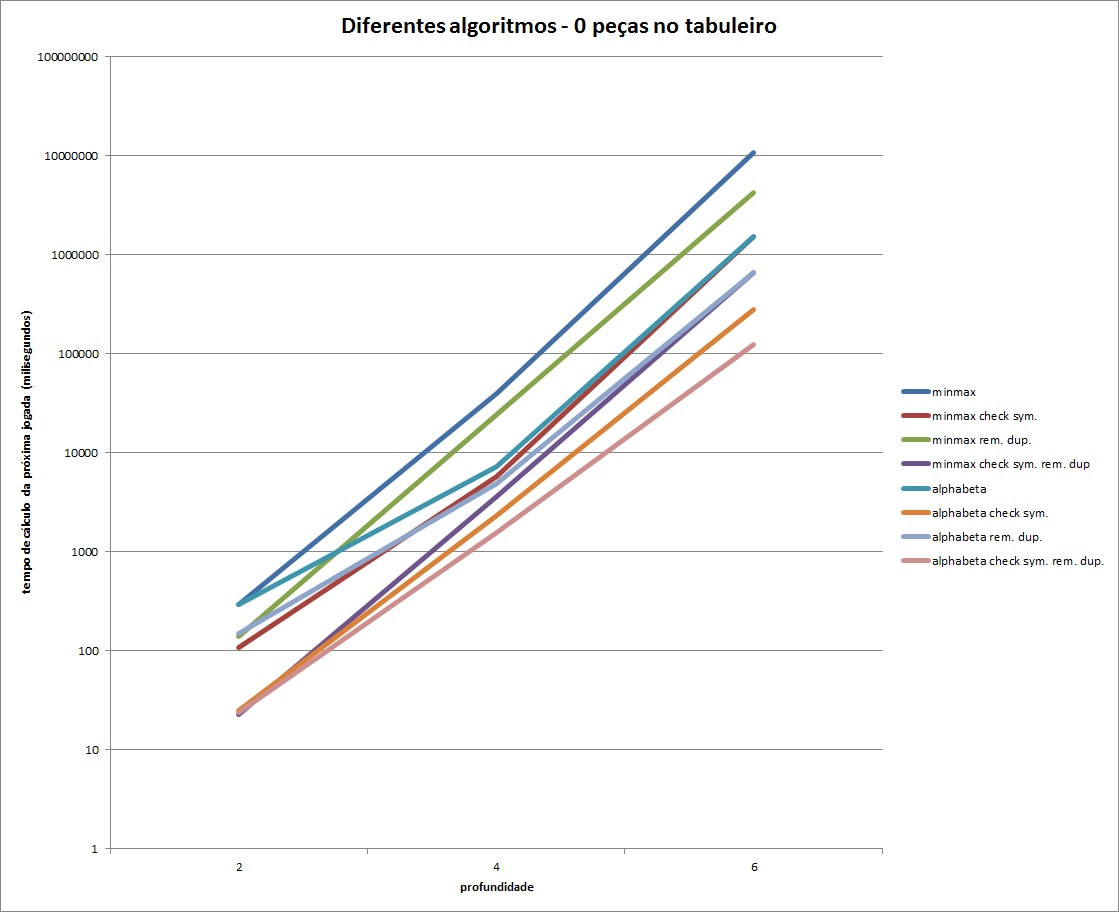
\includegraphics[height=11cm]{performance/tempP0depthComparison.jpg}
\end{table}

O gráfico tem escala logarítmica no eixo dos tempos, daí as retas aproximadas. Isto significa, como já era de esperar, que todos os algoritmos apresentam complexidade exponencial. Também de esperar é a ordenação destes gráficos, sendo a melhor performance do alfa-beta com verificação de simetrias e remoção de duplicados e a pior do minimax sem qualquer melhoria.

\subsubsection{Variação do número de peças}

A variação do número de peças é útil para perceber que se pode obter resultados imediatos com níveis de profundidade diferentes ao longo do jogo. Enquanto que inicialmente o nível de profundidade 4 é o melhor que conseguimos, ao fim de 8 peças, já se consegue praticamente o mesmo tempo com nível de profundidade 6. Além disso, estes testes também ajudam a perceber quando é útil verificar as simetrias e remover duplicados.

\begin{table}[H]
\centering
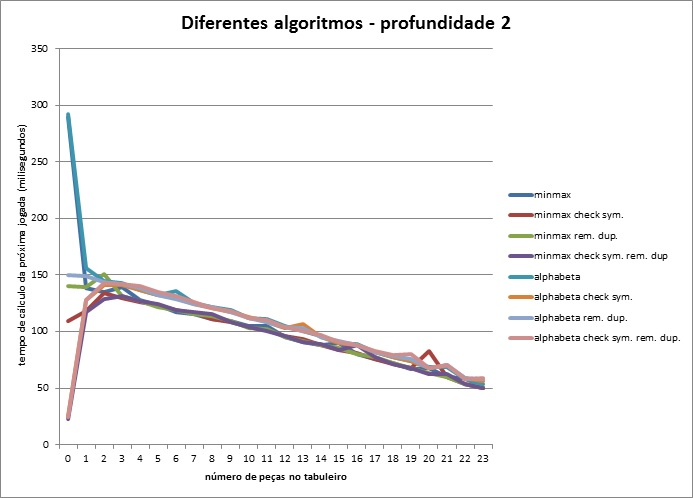
\includegraphics[height=12cm]{performance/tempPerfComparisonDepth2.jpg}
\end{table}

De reparar que a convergência total neste primeiro gráfico se deve ao facto de profundidade 2 corresponder apenas a uma jogada, não existindo por isso cortes alfa-beta.

\begin{table}[H]
\centering
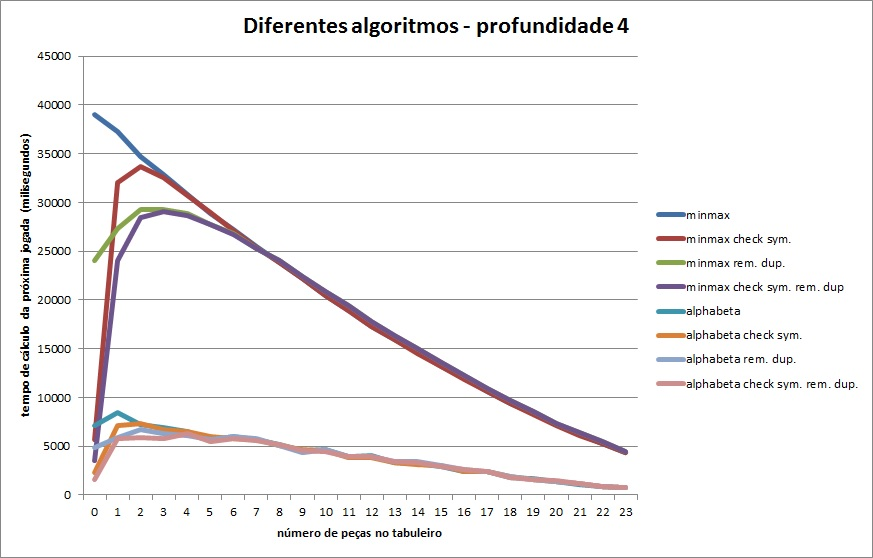
\includegraphics[height=10cm]{performance/tempPerfComparisonDepth4.jpg}
\end{table}

\begin{table}[H]
\centering
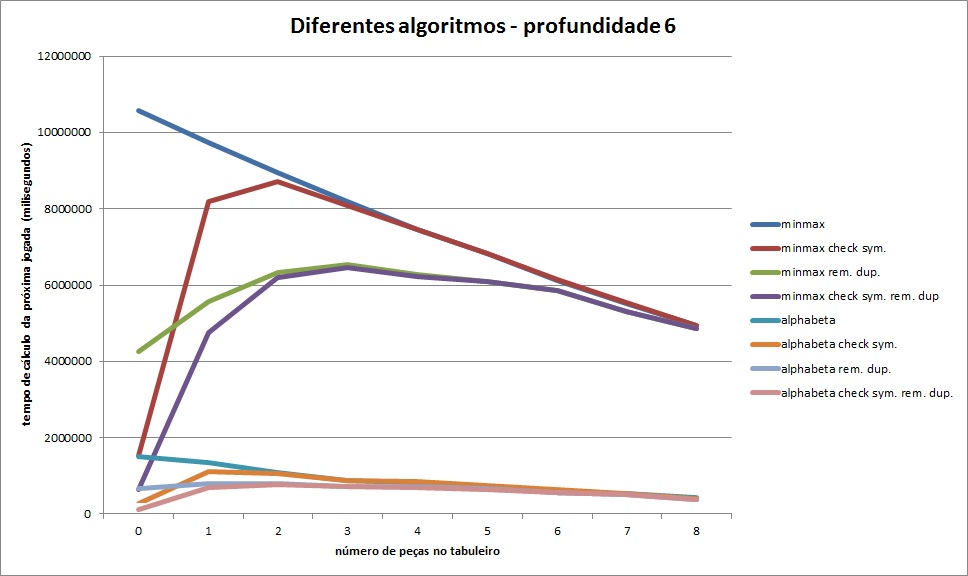
\includegraphics[height=9.5cm]{performance/tempPerfComparisonDepth6.jpg}
\end{table}
